\documentclass{article}

\usepackage{arxiv}

\usepackage[utf8]{inputenc} % allow utf-8 input
\usepackage[T1]{fontenc}    % use 8-bit T1 fonts
\usepackage{lmodern}        % https://github.com/rstudio/rticles/issues/343
\usepackage{hyperref}       % hyperlinks
\usepackage{url}            % simple URL typesetting
\usepackage{booktabs}       % professional-quality tables
\usepackage{amsfonts}       % blackboard math symbols
\usepackage{nicefrac}       % compact symbols for 1/2, etc.
\usepackage{microtype}      % microtypography
\usepackage{graphicx}

\title{Estimating Treatment Effects in Longitudinal Clinical Trials with
Missing Data}

\author{
    Amy Browne
   \\
    Department of Mathemetics \\
    University of Galway \\
   \\
  \texttt{\href{mailto:a.browne47@universityofgalway.ie}{\nolinkurl{a.browne47@universityofgalway.ie}}} \\
   \And
    Tsz Mang Yip
   \\
    Department of Mathemetics \\
    University of Galway \\
   \\
  \texttt{\href{mailto:k.yip2@universityofgalway.ie}{\nolinkurl{k.yip2@universityofgalway.ie}}} \\
  }

% Pandoc syntax highlighting
\usepackage{color}
\usepackage{fancyvrb}
\newcommand{\VerbBar}{|}
\newcommand{\VERB}{\Verb[commandchars=\\\{\}]}
\DefineVerbatimEnvironment{Highlighting}{Verbatim}{commandchars=\\\{\}}
% Add ',fontsize=\small' for more characters per line
\usepackage{framed}
\definecolor{shadecolor}{RGB}{248,248,248}
\newenvironment{Shaded}{\begin{snugshade}}{\end{snugshade}}
\newcommand{\AlertTok}[1]{\textcolor[rgb]{0.94,0.16,0.16}{#1}}
\newcommand{\AnnotationTok}[1]{\textcolor[rgb]{0.56,0.35,0.01}{\textbf{\textit{#1}}}}
\newcommand{\AttributeTok}[1]{\textcolor[rgb]{0.13,0.29,0.53}{#1}}
\newcommand{\BaseNTok}[1]{\textcolor[rgb]{0.00,0.00,0.81}{#1}}
\newcommand{\BuiltInTok}[1]{#1}
\newcommand{\CharTok}[1]{\textcolor[rgb]{0.31,0.60,0.02}{#1}}
\newcommand{\CommentTok}[1]{\textcolor[rgb]{0.56,0.35,0.01}{\textit{#1}}}
\newcommand{\CommentVarTok}[1]{\textcolor[rgb]{0.56,0.35,0.01}{\textbf{\textit{#1}}}}
\newcommand{\ConstantTok}[1]{\textcolor[rgb]{0.56,0.35,0.01}{#1}}
\newcommand{\ControlFlowTok}[1]{\textcolor[rgb]{0.13,0.29,0.53}{\textbf{#1}}}
\newcommand{\DataTypeTok}[1]{\textcolor[rgb]{0.13,0.29,0.53}{#1}}
\newcommand{\DecValTok}[1]{\textcolor[rgb]{0.00,0.00,0.81}{#1}}
\newcommand{\DocumentationTok}[1]{\textcolor[rgb]{0.56,0.35,0.01}{\textbf{\textit{#1}}}}
\newcommand{\ErrorTok}[1]{\textcolor[rgb]{0.64,0.00,0.00}{\textbf{#1}}}
\newcommand{\ExtensionTok}[1]{#1}
\newcommand{\FloatTok}[1]{\textcolor[rgb]{0.00,0.00,0.81}{#1}}
\newcommand{\FunctionTok}[1]{\textcolor[rgb]{0.13,0.29,0.53}{\textbf{#1}}}
\newcommand{\ImportTok}[1]{#1}
\newcommand{\InformationTok}[1]{\textcolor[rgb]{0.56,0.35,0.01}{\textbf{\textit{#1}}}}
\newcommand{\KeywordTok}[1]{\textcolor[rgb]{0.13,0.29,0.53}{\textbf{#1}}}
\newcommand{\NormalTok}[1]{#1}
\newcommand{\OperatorTok}[1]{\textcolor[rgb]{0.81,0.36,0.00}{\textbf{#1}}}
\newcommand{\OtherTok}[1]{\textcolor[rgb]{0.56,0.35,0.01}{#1}}
\newcommand{\PreprocessorTok}[1]{\textcolor[rgb]{0.56,0.35,0.01}{\textit{#1}}}
\newcommand{\RegionMarkerTok}[1]{#1}
\newcommand{\SpecialCharTok}[1]{\textcolor[rgb]{0.81,0.36,0.00}{\textbf{#1}}}
\newcommand{\SpecialStringTok}[1]{\textcolor[rgb]{0.31,0.60,0.02}{#1}}
\newcommand{\StringTok}[1]{\textcolor[rgb]{0.31,0.60,0.02}{#1}}
\newcommand{\VariableTok}[1]{\textcolor[rgb]{0.00,0.00,0.00}{#1}}
\newcommand{\VerbatimStringTok}[1]{\textcolor[rgb]{0.31,0.60,0.02}{#1}}
\newcommand{\WarningTok}[1]{\textcolor[rgb]{0.56,0.35,0.01}{\textbf{\textit{#1}}}}

% tightlist command for lists without linebreak
\providecommand{\tightlist}{%
  \setlength{\itemsep}{0pt}\setlength{\parskip}{0pt}}

% From pandoc table feature
\usepackage{longtable,booktabs,array}
\usepackage{calc} % for calculating minipage widths
% Correct order of tables after \paragraph or \subparagraph
\usepackage{etoolbox}
\makeatletter
\patchcmd\longtable{\par}{\if@noskipsec\mbox{}\fi\par}{}{}
\makeatother
% Allow footnotes in longtable head/foot
\IfFileExists{footnotehyper.sty}{\usepackage{footnotehyper}}{\usepackage{footnote}}
\makesavenoteenv{longtable}


\usepackage{amsmath}
\newcommand{\pandocbounded}[1]{#1}
\begin{document}
\maketitle


\begin{abstract}
\textbf{Motivation} Missing data is a pervasive issue in longitudinal
clinical trials, potentially introducing bias and reducing statistical
power. This project tested different missing data handling techniques,
using two real-world longitudinal randomized clinical trial (RCT)
datasets. \textbf{Results} No substantial differences were observed
between the methods across both datasets.
\textbf{Supplementary Information} Code is available at
\url{https://github.com/amydebrun/Missing-Data}.
\end{abstract}

\keywords{
    Missing Data
   \and
    Longitudinal Data
   \and
    Randomized Clinical Trial
   \and
    Real World Data Analysis
   \and
    Sensitivity Analysis
   \and
    Multiple Imputation
   \and
    Missingness Mechanisms
  }

\newpage

\section{Introduction - amy}\label{introduction---amy}

\subsection{Missing data in longitudinal
study}\label{missing-data-in-longitudinal-study}

\emph{Longitudinal Study Design}

Longitudinal studies are research designs in which data are collected
from the same participants at multiple time points. They provide
valuable insights into how variables change over time---often over
several years or decades. While this design is powerful for
understanding causal relationships and long-term trends, it presents
significant challenges in retaining participants across all waves of
data collection.

Longitudinal trials require consistent data collection methods at
predefined intervals. Researchers must work to minimize participant
dropout or non-response. However, due to the extended duration and
complexity of these studies, missing data is almost inevitable.

Similarly, clinical trials which evaluate the effects of biomedical or
behavioral interventions are also vulnerable to missing data.
Participants may miss follow-ups due to illness or other commitments.
This loss of data can compromise the study's validity. Ignoring missing
data introduces bias, as we're disregarding potentially informative
cases. For instance, if participants drop out due to adverse effects
from the treatment, the missing data is not random---this introduces
attrition bias, which can distort estimates of the treatment's effect.

Removing incomplete cases reduces the sample size, which in turn
decreases statistical power, limiting the ability to detect valid
treatment effects.

In statistical software like R, missing values are represented as NA.
When fitting models like linear regression, R automatically excludes any
subjects with missing values in either predictor or outcome variables.
While convenient, this method can lead to selection bias if the
missingness is systematic.

\subsection{Project Objective}\label{project-objective}

The objective of this project is to estimate treatment effects using
real-world data, with a primary focus on addressing issues that come
with missing data. We will briefly discuss different assumptions about
missing data mechanisms---such as Missing Completely at Random, Missing
at Random, and Missing Not at Random and investigate their implications
for statistical analysis.

While a range of methods are available to handle missing data, they all
vary in levels of complexity and assumptions. This project aims to
explore these methods, understand the reasons behind their differing
performance, and implement them on real-world longitudinal clinical data
to compare their effectiveness in estimating treatment effects.

After initial exploration of the different methods, we also decided to
adjust the estimands through data wrangling our chosen datasets to
compare how the estimate differs when the estimand is either categorical
or continuous and to compare the effects using linear regression or
linear mixed effects models. Additionally, we will conduct sensitivity
analyses to investigate how treatment effect estimates change under
different assumptions about the missing data.

\subsection{Missingness Mechanisms}\label{missingness-mechanisms}

Missing data mechanisms are important to consider when choosing which
sort of missing data handling method to use. There are three mechanisms
which missing data can follow:

\begin{itemize}
\tightlist
\item
  Missing Completely At Random (MCAR)
\item
  Missing At Random (MAR)
\item
  Missing Not At Random (MNAR)
\end{itemize}

Although they may appear similar at first glance, continuing to handle
missing data without considering these mechanisms may still result in
biased estimates and inaccurate conclusions. Missing data mechanisms
appear to be mentioned first by Donald Rubin in 1976. We can formally
define these mechanisms using the following notation;

\begin{itemize}
\tightlist
\item
  \(R\) represents a missing data indicator which when \(R=1\) indicates
  observed data and \(R=0\) indicates unobserved
\item
  \(X\) represents data that is always observed
\item
  \(Y\) represents data that is potentially missing.
\end{itemize}

\textbf{Missing Completely At Random}

The formal definition of MCAR data is:

\[\quad P(R = 1 \mid Y, X) = P(R = 1)\] The probability of the data is
observed given observed data and missing data is the same as the
probability of being observed without the given data. This mechanism is
considered the easiest to deal with as it does not bias the result
although data is rarely MCAR. This can occur due to system failure and
some data is deleted accidentally, or else there is issues with the
treatment system and data cannot be recorded. The DAG below visualises
an example of this mechanism based on a randomised trial with
randomisation variable \(L\). Missing indicator \(R\), which denotes
whether the outcome is observed (\(R = 1\)) or missing (\(R = 0\)), is
independent from the observed baseline variables \(X1\) and \(X2\) and
outcome variable \(Y\) (which contains potentially missing data).

\pandocbounded{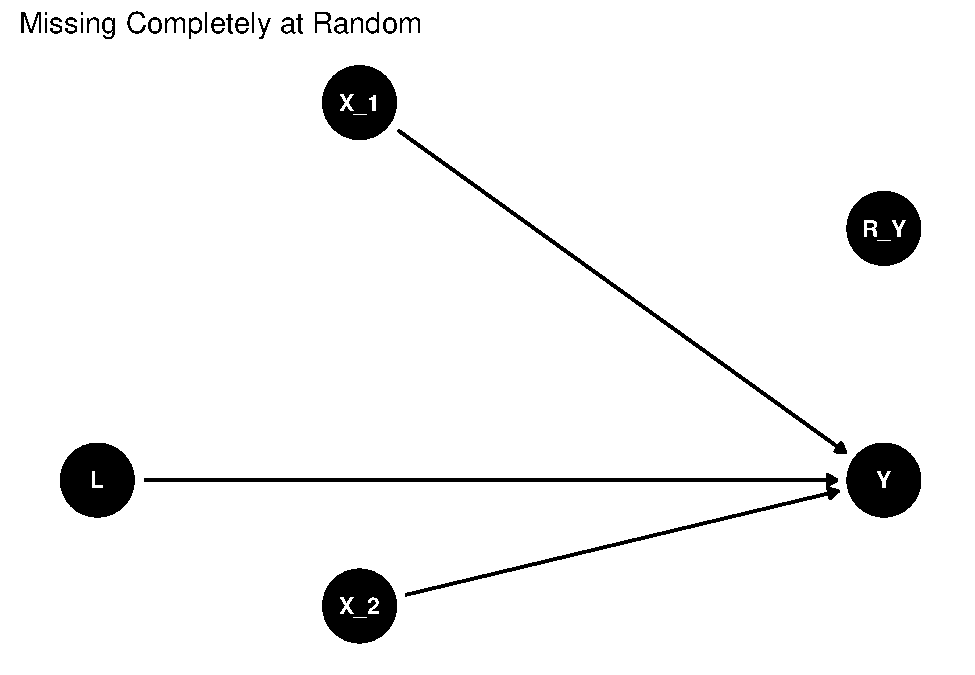
\includegraphics[keepaspectratio]{Final_Report_files/figure-latex/unnamed-chunk-1-1.pdf}}

\textbf{Missing At Random}

\[\quad P(R = 1 \mid Y, X) = P(R = 1 \mid X)\] The probability of data
being observed given the rest of the data is the same as the probability
being observed given the observed data. In short, the data's missingness
is dependent on the observed data. For example, people with a higher
body mass index may be more prone to having missing blood pressure data
- this is not relative to the missing data. MAR is a more realistic
mechanism than MCAR and requires more intensive handling methods. The
DAG shows that the \(R\) is influenced by the \(Y\), \(X1\), \(X2\) and
treatment \(A\).

\pandocbounded{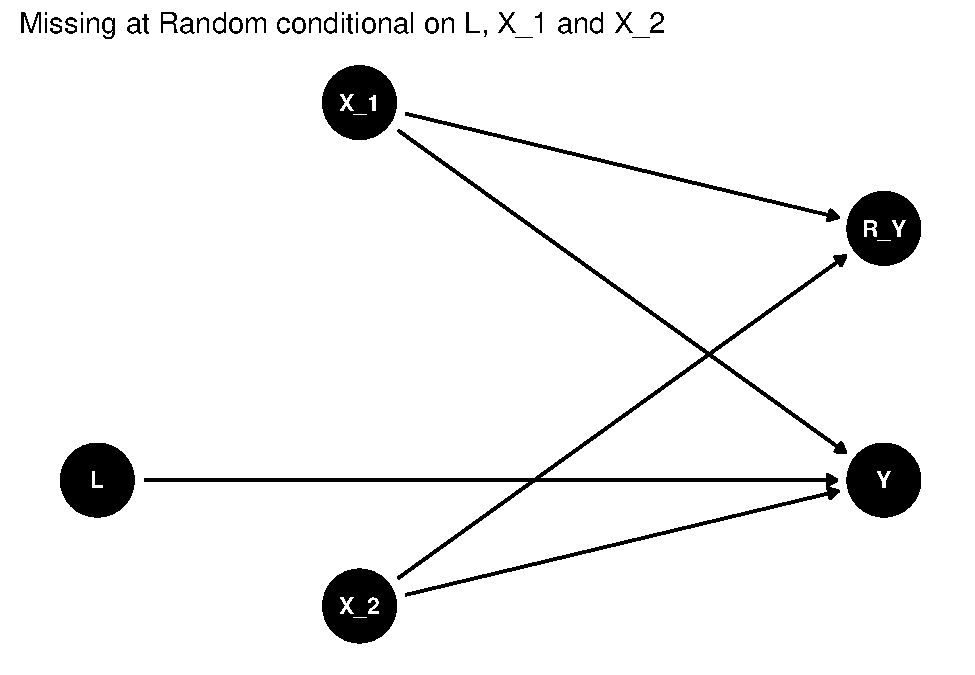
\includegraphics[keepaspectratio]{Final_Report_files/figure-latex/unnamed-chunk-2-1.pdf}}

\textbf{Missing Not At Random}

\[\quad P(R = 1 \mid Y, X) \ne P(R = 1 \mid X)\] The probability of data
being observed is not dependent on the observed data. This mechanism is
the most difficult to deal with as it relates to the unobserved data, so
producing valid results is a challenge. Certain participants in a
general health study may avoid answering questions truthfully about
smoking habits or their diet in order to make themselves more appealing.
Sensitivity analysis is an option to determine the treatment effect when
assuming different mechanisms. The following DAG includes the missing
data indicator \(R\). In this structure, the potentially missing outcome
variable \(Y\) directly influences \(R\).

\pandocbounded{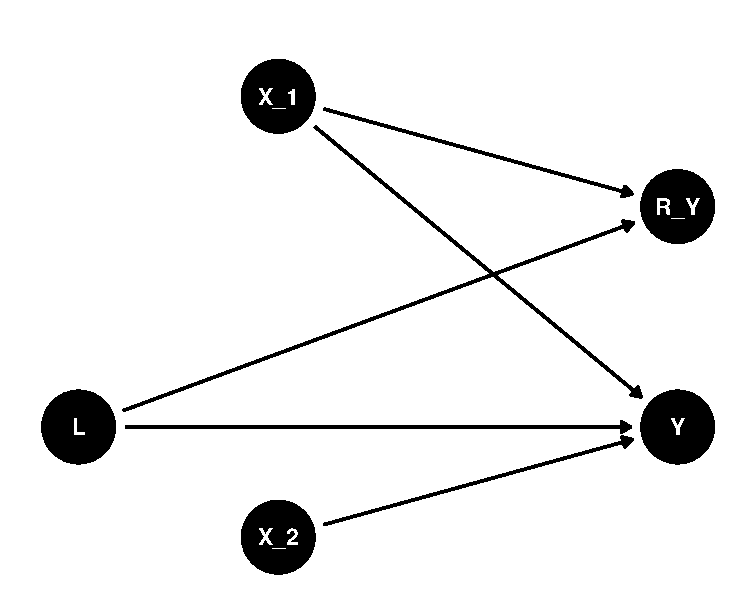
\includegraphics[keepaspectratio]{Final_Report_files/figure-latex/unnamed-chunk-3-1.pdf}}

Although these considerations are important, the mechanism underlying
missing data is fundamentally untestable. Since the true values of
missing observations are never observed, we cannot definitively
determine which missingness assumption holds in practice. There is
limited hypothesis test available to see whether data is MCAR
(\emph{Little's MCAR test}). It is a likelihood-ratio test that groups
missing data patterns, estimates the expected means under a multivariate
normal model using maximum likelihood, and computes a chi-square
statistic to assess model fit. It is limited as it does not necessarily
confirm MCAR but provides no evidence to reject that the data MCAR. If
the test has a significant p-value, it suggests that the data is MAR or
MNAR, but we do not know which one.

\subsection{Different missing data patterns (section
tbc)}\label{different-missing-data-patterns-section-tbc}

A missing data pattern describes the pattern of missing data among the
observed data. As described by Little \& Rubin (2014), it's important to
remark the missing data patterns of the data set prior to data handling
as some handling methods are intended for certain classified patterns.

\begin{verbatim}
## # A tibble: 6 x 2
##   `Missing Data Pattern` Description                                            
##   <chr>                  <chr>                                                  
## 1 Univariate             "Missing values in a single variable"                  
## 2 Multivariate           "Missing values present in multiple variables"         
## 3 Monotonic              "variables $Y_j$ can be ordered if missing"            
## 4 General                "Missing valueshave no structure and scattered through~
## 5 File Matching          "Missing data appears to be statistically matched"     
## 6 Factor Analysis        ""
\end{verbatim}

\subsection{Literature and
Limitations}\label{literature-and-limitations}

While reviewing the literature on missing data, it became evident that
despite the use of established handling methods, there remains room for
improvement in how missing data are addressed in reports and in the
selection of appropriate methods.

In 2014, Powney et al.~reviewed 100 longitudinal clinical trials
conducted between 2005 and 2012 and found that only 44 reported an
adequate method to handle missing data, while 30 used potentially
inadequate methods.

Spineli et al.~(2015) examined 190 systematic reviews published after
2009 to investigate how missing data were reported in randomized
controlled trials. Although 175 of these reviews mentioned missing data,
only 61 discussed its implications.

Hunt et al.~(2021) reviewed 62 pharmacoepidemiologic multi-database
studies from 2018 to 2019 to assess missing data reporting and handling.
Thirty-five studies reported missing data, but only 19 described methods
for handling it. The most popular approach was complete case analysis
(CCA) used in 13 studies, followed by multiple imputation (MI) in 2
studies.

Complete case analysis was also the predominant method in a systematic
review of 229 observational studies from the United Network for Organ
Sharing (UNOS) database (Baker et al., 2025). Forty-one studies used
CCA, 22 reported MI, and notably, 31 studies removed covariates due to
missing values---an action that could introduce further bias depending
on the covariates' relationship with other predictors.

\newpage

\section{Real World Data}\label{real-world-data}

We have sourced two different data sets to perform our missingness
analysis on. They both have different sample sizes and different levels
of missing data which is an advantage as we can conduct analysis in
different settings.

\textbf{Acupuncture Data}

\emph{Source}

Vickers et al.~published a paper in 2004 on a trial they conducted to
determine the effect of acupuncture therapy on chronic headache in
primary care. Vickers released the dataset from the study in 2006 and is
publicly available to download in excel format from
\url{https://pmc.ncbi.nlm.nih.gov/articles/PMC1489946/}.

\emph{Study Design}

The study design for the acupuncture trial is a longitudinal randomised
controlled trial with two follow up time points. 401 participants were
gathered from general practices in England and Wales who suffered from
migraines.

\emph{Data Overview}

13 variables were recorded during the acupuncture trial.

\begin{verbatim}
## # A tibble: 14 x 2
##    Variable      Description                                     
##    <chr>         <chr>                                           
##  1 id            patient ID code                                 
##  2 age           Age                                             
##  3 sex           sex; female (1) vs. male (0)                    
##  4 migraine      diagnosis ; migraine (1) vs. tension-type (0)   
##  5 chronicity    number of years of headache disorder            
##  6 acupuncturist acupuncturist id code                           
##  7 practice_id   gp practice id                                  
##  8 group         treatment group; acupuncture (1) vs. control (0)
##  9 pk1           headache severity score baseline                
## 10 pk2           headache severity score 3 month                 
## 11 pk5           headache severity score 1 year                  
## 12 f1            headache frequency baseline                     
## 13 f2            headache frequency 3 month                      
## 14 f5            headache frequency 1 year
\end{verbatim}

Variables \texttt{pk2} and `\texttt{pk5} are the follow-up times at 3
months and 12 months.

\begin{verbatim}
## 
## 
## |**Characteristic** | **0**  N = 196 | **1**  N = 205 |
## |:------------------|:--------------:|:--------------:|
## |id                 |   470 (209)    |   472 (206)    |
## |age                |    45 (11)     |    46 (11)     |
## |sex                |    165(84%)    |    172(84%)    |
## |migraine           |    183(93%)    |    194(95%)    |
## |chronicity         |    22 (13)     |    21 (14)     |
## |acupuncturist      |  5.97 (2.82)   |  6.00 (2.80)   |
## |practice_id        |    24 (11)     |    25 (12)     |
## |pk1                |    27 (17)     |    26 (15)     |
## |pk2                |    24 (18)     |    19 (16)     |
## |Missing            |       43       |       32       |
## |pk5                |    22 (17)     |    16 (14)     |
## |Missing            |       56       |       44       |
## |f1                 |     16 (7)     |     16 (7)     |
## |f2                 |     11 (9)     |     11 (8)     |
## |f5                 |     10 (9)     |     9 (8)      |
\end{verbatim}

Figure 2.x is the summary statistics of the acupuncture trial data. Note
pk2 and pk5 are post randomisation variables and contain missing data.

\pandocbounded{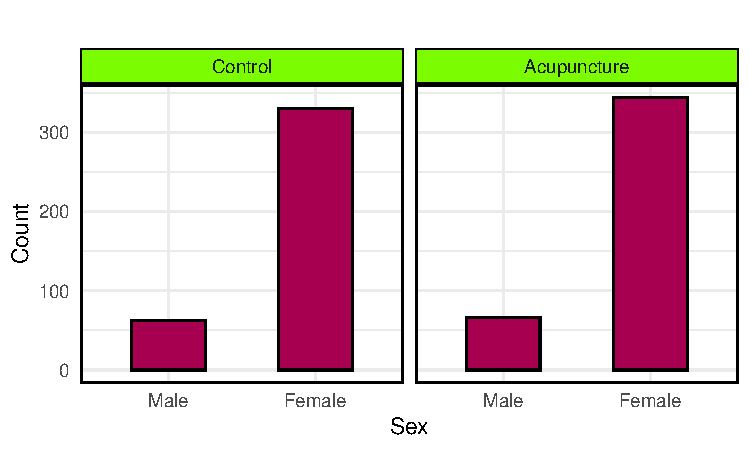
\includegraphics[keepaspectratio]{Final_Report_files/figure-latex/unnamed-chunk-7-1.pdf}}

Figure 2.x is the distribution of sex in both treatment groups of the
acupuncture trial data. The participants are predominantly female.

\pandocbounded{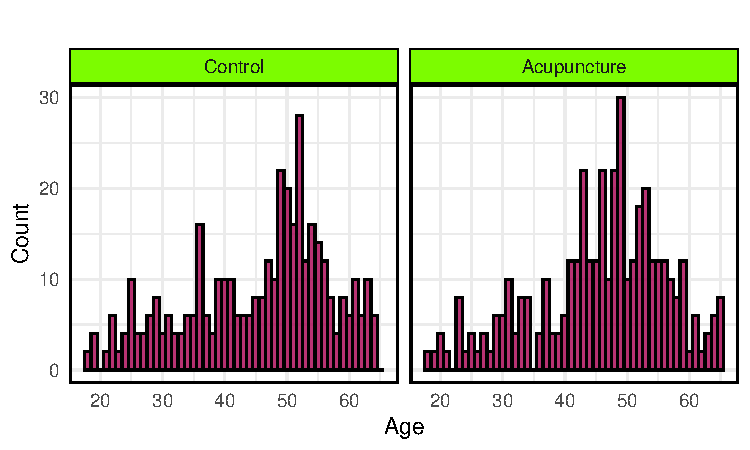
\includegraphics[keepaspectratio]{Final_Report_files/figure-latex/unnamed-chunk-8-1.pdf}}

Figure 2.x is the distribution of age in both treatment groups. Both
distributions are negatively skewed, predominantly middle aged and
older.

\pandocbounded{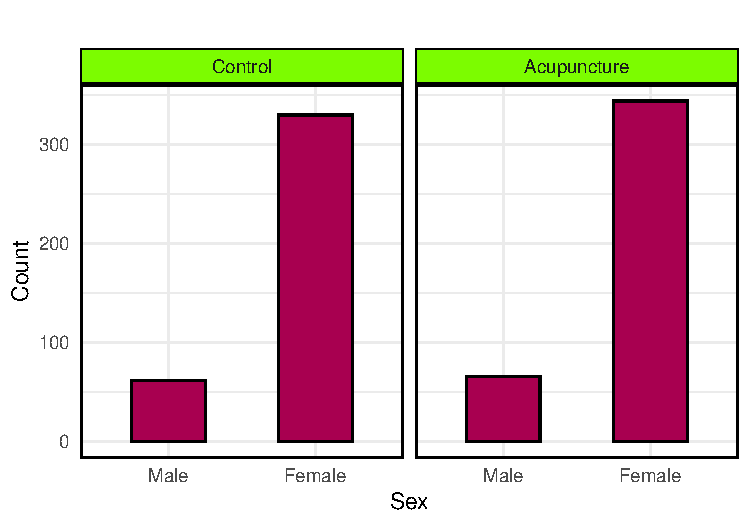
\includegraphics[keepaspectratio]{Final_Report_files/figure-latex/unnamed-chunk-9-1.pdf}}

\pandocbounded{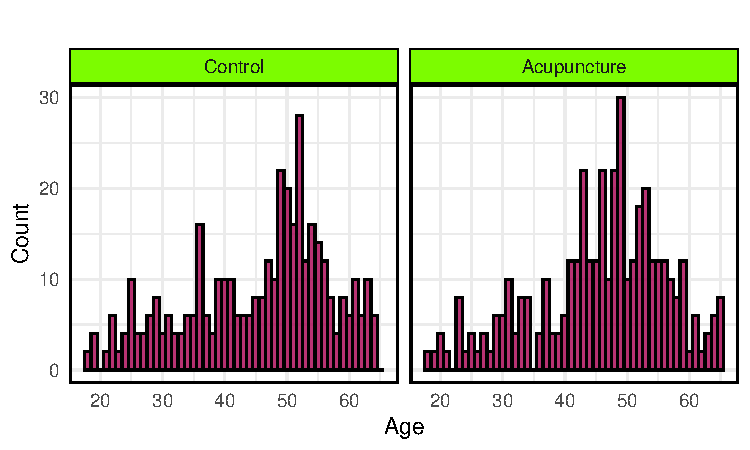
\includegraphics[keepaspectratio]{Final_Report_files/figure-latex/unnamed-chunk-10-1.pdf}}

\pandocbounded{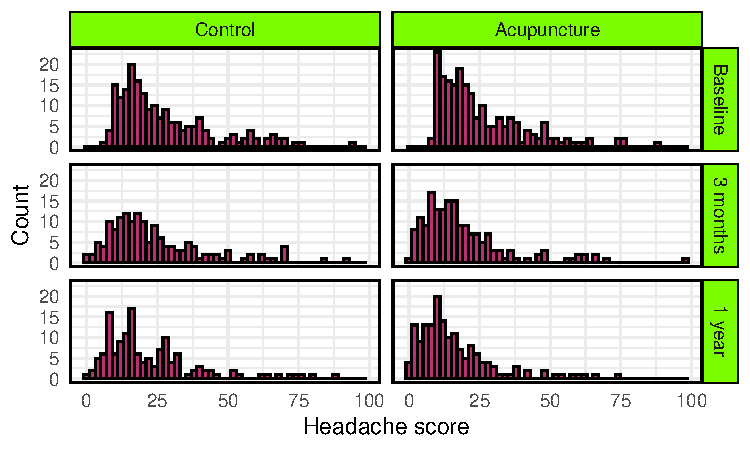
\includegraphics[keepaspectratio]{Final_Report_files/figure-latex/unnamed-chunk-11-1.pdf}}

Figure 2.x,2.x,2.x: These plots show the distribution of the headache
severity score at the three measured time-points. Over the three
time-points we can see a generally positively skewed distribution with
most headache severity scores ranging between 0 and 35. There appears to
be minimal difference in headache severity score over the treatment
group, and the control group appears to have a lower headache severity
score overall. The 3 month and 12 month time-point distributions are
incomplete due to the missing values.

\emph{Original Estimand}

The aim of the original study was to estimate the effect of acupuncture
therapy on chronic headache in comparison to general care. Therefore,
our estimand with the sourced data set is the difference in mean
headache score at the final time point of 12 months between the
acupuncture group and the control group. This is modelled parsimoniously
by

\[\text{pk5}_i = \beta_0 + \beta_1 \text{group}_i + \beta_2 \text{pk1}_i + \varepsilon_i\]
where

\begin{itemize}
\tightlist
\item
  \(pk5_i\) is the headache severity of individual \(i\) at 12 months.
\item
  \(\beta_0\) is our intercept parameter when there is no treatment
  group and no recorded baseline headache severity.
\item
  \(\beta_1\) is the effect of the treatment group. This is our
  treatment effect of interest.
\item
  \(\beta_2\) is the effect of the baseline headache severity
\item
  \(\varepsilon_i\) is the residual error term for individual \(i\)
\end{itemize}

\textbf{VITAL data}

\emph{Source}

MacFarlane et al.~conducted a study on the therapeutic effects of
vitamin D and fish oil on osteoarthritic knee pain. We sourced this data
at xyz.

\emph{Study Design}

This study was a 2x2 factorial designed longitudinal randomised
controlled trial. 1,398 participants in the study was randomised to 4
possible treatment combinations. Participants were randomised to receive
either omega-3 oils or vitamin D, both treatments, or randomised to the
placebo group. For this research project, we assumed that that the
participants were only randomised to either receive the fish oil
treatment, vitamin D treatment or the placebo. We did not include the
interaction between vitamin D and fish oil in our substantive model or
our imputation model.

\begin{longtable}[]{@{}lll@{}}
\toprule\noalign{}
& \textbf{Vitamin D} & \textbf{Placebo} \\
\midrule\noalign{}
\endhead
\bottomrule\noalign{}
\endlastfoot
\textbf{Fish Oil} & N = 342 \emph{(not analysed)} & N = 353 \\
\textbf{Placebo} & N = 332 & N = 371 \\
\end{longtable}

\emph{Data Overview}

There are x variables recorded in the VITAL data, the following table
refers to a subset of the variables that we frequently use.

\begin{verbatim}
## # A tibble: 13 x 2
##    Variable       Description                              
##    <chr>          <chr>                                    
##  1 Subject_ID     Patient ID code                          
##  2 age            Age of patient                           
##  3 bmi            Body mass index of patient               
##  4 sex            Sex of patient                           
##  5 vitdactive     1=vitamin D, 0=no vitamin D              
##  6 fishoilactive  1= fish oil, 0= no fish oil              
##  7 pain_base      Knee pain at baseline                    
##  8 pain_yrX       Knee pain X years post randomisation     
##  9 stiffness_base Knee stiffness at baseline               
## 10 stiffness_yrX  Knee stiffness X years post randomisation
## 11 function_base  Knee function at baseline                
## 12 function_yrX   Knee function X years post randomisation 
## 13 kneepainfreq   Frequency of knee pain
\end{verbatim}

\begin{verbatim}
## 
## 
## |**Characteristic**                                                             | **Both**  N = 342 | **Fish Oil only**  N = 353 | **Neither**  N = 371 | **Vitamin D only**  N = 332 |
## |:------------------------------------------------------------------------------|:-----------------:|:--------------------------:|:--------------------:|:---------------------------:|
## |Sex 1-male,2-female                                                            |                   |                            |                      |                             |
## |1                                                                              |     111(32%)      |          120(34%)          |       123(33%)       |          124(37%)           |
## |2                                                                              |     231(68%)      |          233(66%)          |       248(67%)       |          208(63%)           |
## |Body mass index at randomization, kg/m2                                        |      32 (7)       |           32 (7)           |        32 (8)        |           31 (7)            |
## |Missing                                                                        |         8         |             11             |          14          |             12              |
## |Current smoking 1-yes,0-no                                                     |     26(7.8%)      |          33(9.4%)          |       30(8.2%)       |          22(6.8%)           |
## |Missing                                                                        |         7         |             2              |          3           |              8              |
## |Age at randomization to VITAL study,years                                      |      67 (7)       |           67 (7)           |        68 (7)        |           67 (6)            |
## |Baseline Aspirin use 1-yes,0-no                                                |     156(46%)      |          165(47%)          |       176(48%)       |          155(48%)           |
## |Missing                                                                        |         6         |             5              |          6           |              7              |
## |WOMAC Pain score at baseline                                                   |      37 (19)      |          37 (18)           |       37 (19)        |           36 (18)           |
## |Missing                                                                        |        48         |             57             |          45          |             40              |
## |WOMAC Pain score at year 1                                                     |      32 (19)      |          31 (20)           |       33 (20)        |           33 (21)           |
## |Missing                                                                        |        182        |            162             |         184          |             153             |
## |WOMAC Pain score at year 2                                                     |      32 (20)      |          31 (20)           |       30 (20)        |           32 (20)           |
## |Missing                                                                        |        47         |             46             |          48          |             47              |
## |WOMAC Pain score at year 3                                                     |      32 (21)      |          31 (19)           |       31 (19)        |           28 (19)           |
## |Missing                                                                        |        78         |             95             |          90          |             82              |
## |WOMAC Pain score at year 4                                                     |      30 (20)      |          30 (19)           |       29 (18)        |           28 (19)           |
## |Missing                                                                        |        129        |            149             |         145          |             126             |
## |Have you had a knee replacement surgery? (1=Yes, 2=No)                         |                   |                            |                      |                             |
## |1                                                                              |      43(13%)      |          47(14%)           |       52(14%)        |           53(16%)           |
## |2                                                                              |     293(87%)      |          300(86%)          |       316(86%)       |          271(84%)           |
## |Missing                                                                        |         6         |             6              |          3           |              8              |
## |Unilateral knee pain 1=Yes 0=No                                                |     200(71%)      |          198(69%)          |       223(72%)       |          200(71%)           |
## |Missing                                                                        |        61         |             68             |          61          |             49              |
## |Bilateral knee pain 1=Yes 0=No                                                 |      81(29%)      |          87(31%)           |       87(28%)        |           83(29%)           |
## |Missing                                                                        |        61         |             68             |          61          |             49              |
## |Frequency of knee pain 1=Never 2=<1 day/wk 3=1~2 days/wk 4=3~6 days/wk 5=daily |                   |                            |                      |                             |
## |1                                                                              |      1(0.3%)      |          1(0.3%)           |       2(0.6%)        |           1(0.3%)           |
## |2                                                                              |     16(5.4%)      |          19(6.4%)          |       11(3.3%)       |          16(5.4%)           |
## |3                                                                              |      44(15%)      |          27(9.0%)          |       34(10%)        |           31(10%)           |
## |4                                                                              |      58(20%)      |          57(19%)           |       68(21%)        |           57(19%)           |
## |5                                                                              |     169(57%)      |          185(62%)          |       201(61%)       |          181(61%)           |
## |9                                                                              |      7(2.4%)      |          10(3.3%)          |       14(4.2%)       |          10(3.4%)           |
## |Missing                                                                        |        47         |             54             |          41          |             36              |
## |Tylenol use at baseline 1=never 2=occational 3=daily 9=missing                 |                   |                            |                      |                             |
## |1                                                                              |     108(37%)      |          137(46%)          |       145(44%)       |          135(46%)           |
## |2                                                                              |      91(31%)      |          84(28%)           |       110(33%)       |           95(32%)           |
## |3                                                                              |      53(18%)      |          41(14%)           |       38(12%)        |           30(10%)           |
## |9                                                                              |      43(15%)      |          37(12%)           |       37(11%)        |           36(12%)           |
## |Missing                                                                        |        47         |             54             |          41          |             36              |
## |Nsaids use at baseline 1=never 2=occational 3=daily 9=missing                  |                   |                            |                      |                             |
## |1                                                                              |      62(21%)      |          65(22%)           |       69(21%)        |           73(25%)           |
## |2                                                                              |      98(33%)      |          101(34%)          |       98(30%)        |           94(32%)           |
## |3                                                                              |     110(37%)      |          107(36%)          |       134(41%)       |          111(38%)           |
## |9                                                                              |     25(8.5%)      |          26(8.7%)          |       29(8.8%)       |          18(6.1%)           |
## |Missing                                                                        |        47         |             54             |          41          |             36              |
## |Stronger med use at baseline 1=never 2=occational 3=daily 9=missing            |                   |                            |                      |                             |
## |1                                                                              |     178(60%)      |          193(65%)          |       205(62%)       |          186(63%)           |
## |2                                                                              |      40(14%)      |          41(14%)           |       43(13%)        |           47(16%)           |
## |3                                                                              |      46(16%)      |          36(12%)           |       50(15%)        |           40(14%)           |
## |9                                                                              |      31(11%)      |          29(9.7%)          |       32(9.7%)       |          23(7.8%)           |
## |Missing                                                                        |        47         |             54             |          41          |             36              |
## |TKR 1=yes 0=No                                                                 |      64(19%)      |          82(23%)           |       74(20%)        |           76(23%)           |
\end{verbatim}

Figure 2.x shows the summary statistics of the VITAL data. It provides
information on all 4 treatment groups. Note here that the VITAL data
contains missing baseline data as well as post randomisation data.

\begin{center}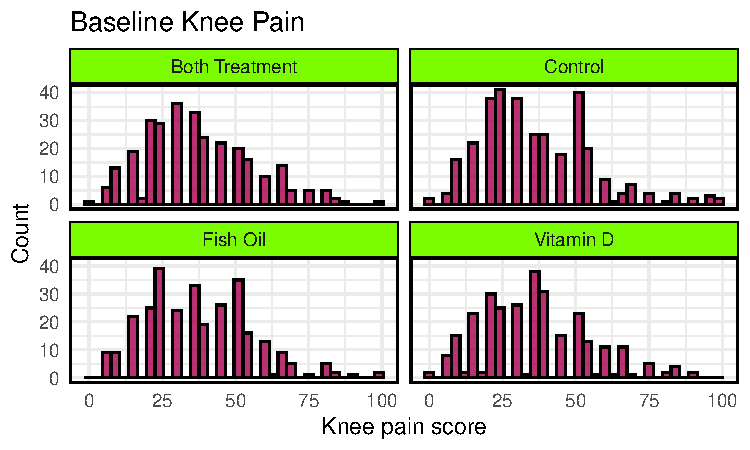
\includegraphics{Final_Report_files/figure-latex/unnamed-chunk-14-1} \end{center}

Figure 2.x shows the distribution of age in each treatment group, which
appear to be normal/ positive skewed distributions.

\begin{center}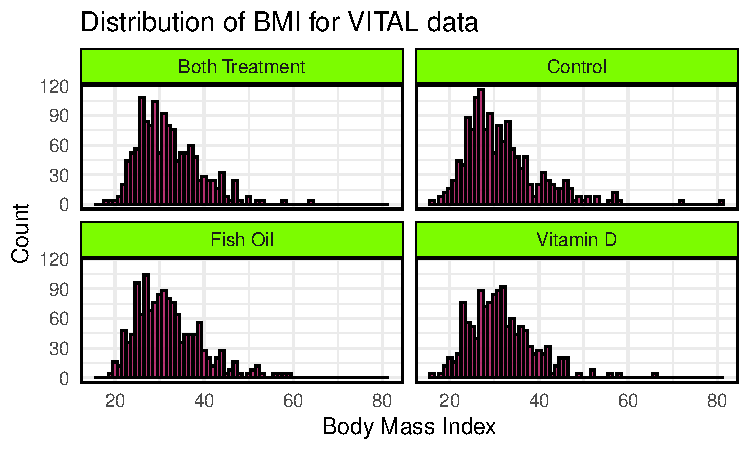
\includegraphics{Final_Report_files/figure-latex/unnamed-chunk-15-1} \end{center}

Figure 2.x shows the distribution of body mass index in each treatment
group, these appear to be positively skewed with a bmi between 20 and
40. This shows a range between healthy weighted and obese participants.

\pandocbounded{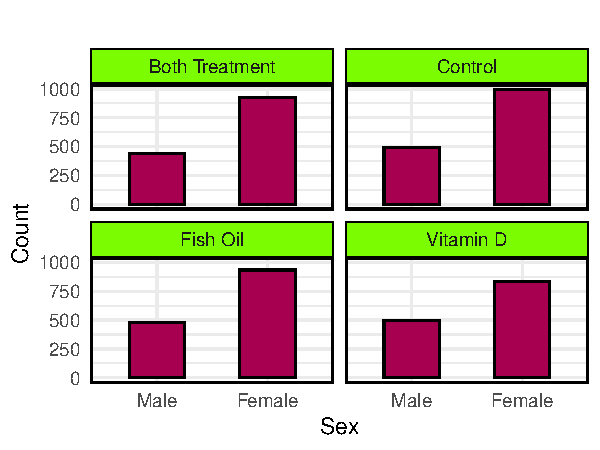
\includegraphics[keepaspectratio]{Final_Report_files/figure-latex/unnamed-chunk-16-1.pdf}}

Figure 2.x is the distribution of males and females in the VITAL data.
Similar to the acupuncture trial, the participants are predominantly
female.

\pandocbounded{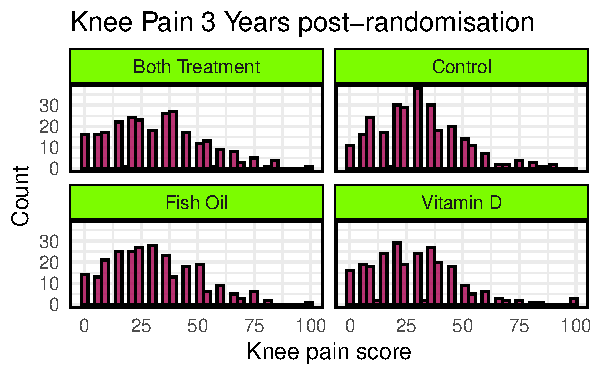
\includegraphics[keepaspectratio]{Final_Report_files/figure-latex/unnamed-chunk-17-1.pdf}}

\pandocbounded{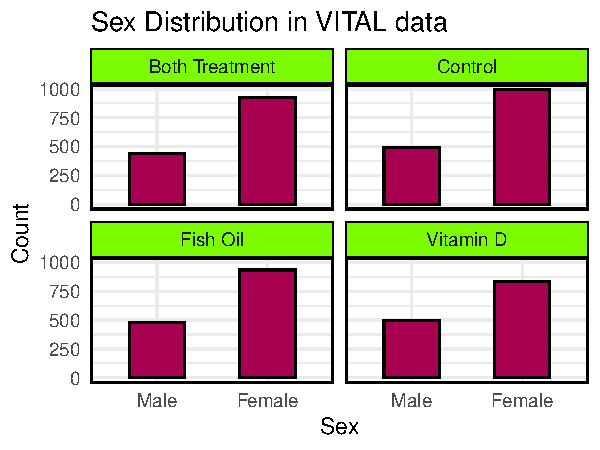
\includegraphics[keepaspectratio]{Final_Report_files/figure-latex/unnamed-chunk-18-1.pdf}}

\pandocbounded{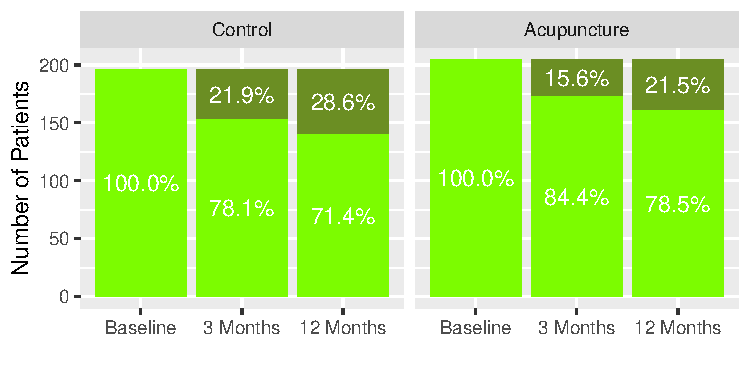
\includegraphics[keepaspectratio]{Final_Report_files/figure-latex/unnamed-chunk-19-1.pdf}}

\pandocbounded{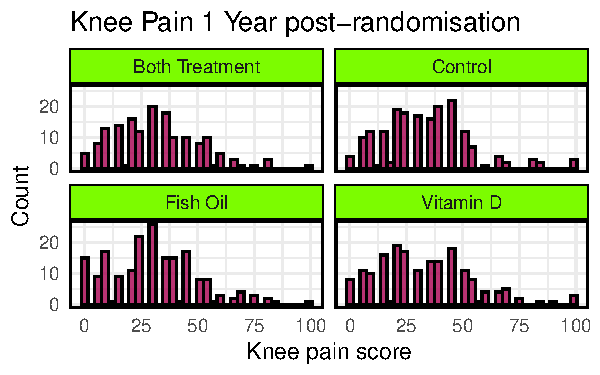
\includegraphics[keepaspectratio]{Final_Report_files/figure-latex/unnamed-chunk-20-1.pdf}}

\pandocbounded{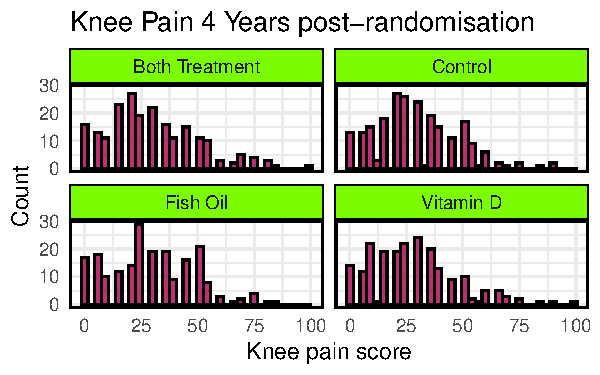
\includegraphics[keepaspectratio]{Final_Report_files/figure-latex/unnamed-chunk-21-1.pdf}}

Figure 2.x,2.x,2.x,2.x,2.x shows the distribution of the knee pain from
baseline until 4 years post randomisation. In all treatment groups it
appears that the distributions follow a positive/ near normal
distribution and skews more positive as time goes on. This occurs in all
groups. Each time-point has an incomplete distribution due to missing
data.

\emph{Original estimand in VITAL study}

Our estimand for this dataset is the difference in mean knee pain at the
final time point of 4 years post randomisation \(pain_yr4\) which is
modelled by
\[painyear4_i = \beta_0 + \beta_1 fishoilactive_i + \beta_2 vitdactive_i + \beta_3 painbase_i + \varepsilon_i\]
in which

\begin{itemize}
\tightlist
\item
  \(text{pain_yr4}_i\) is the knee pain score for individual \(i\) at
  the final time point of 4 years post randomisation.
\item
  \(\beta_0\) is the intercept parameter which represents the knee pain
  score when there is no treatment of vitamin D or fish oil given and no
  baseline knee pain score is recorded.
\item
  \(\beta_1\) is the effect of being randomised to the fishoil treatment
  group. This is the treatment effect of interest in our fishoil only
  missingness analysis.
\item
  \(\beta_2\) is the effect of being randomised to the vitamin D
  treatment group. This is the treatment effect of interest in our
  vitamin D only missingness analysis.
\item
  \(\beta_3\) is the effect of the baseline knee pain score
  pre-randomisation.
\item
  \(\varepsilon\) is the residual error of individual \(i\)
\end{itemize}

\newpage

\subsection{Missing analysis}\label{missing-analysis}

\textbf{Acupuncture Data}

The summary statistics of the acupuncture trial data shows that all
baseline variables have been observed. It appears two post-randomisation
outcome variables contain missing data. This pattern would be described
as a multivariate monotonic pattern as the percentage of missing data
increases at each follow up time point, which is common in longitudinal
studies. We can visualise this in the plot below.

\pandocbounded{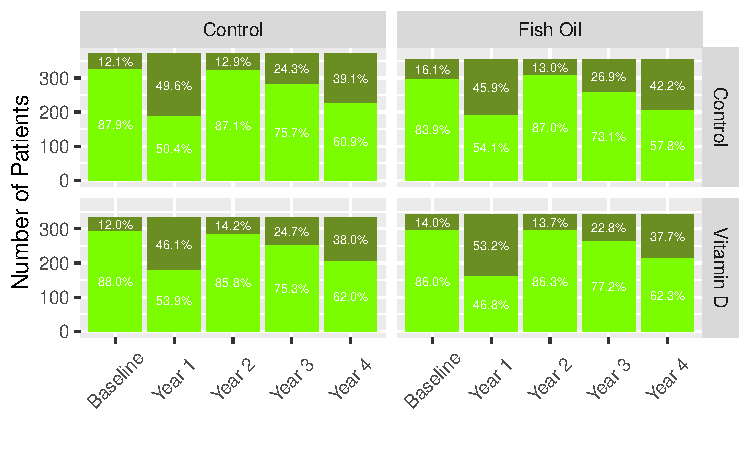
\includegraphics[keepaspectratio]{Final_Report_files/figure-latex/unnamed-chunk-22-1.pdf}}

Figure 2.x: Proportion of missing data (dark green) in outcome variables
\(pk2\) and \(pk5\). This follows a monotonic missing data pattern.

If we separate the acupuncture trial data into the treatment group and
control group, we can observe that there is a higher percentage of
missing data in the control group.

\pandocbounded{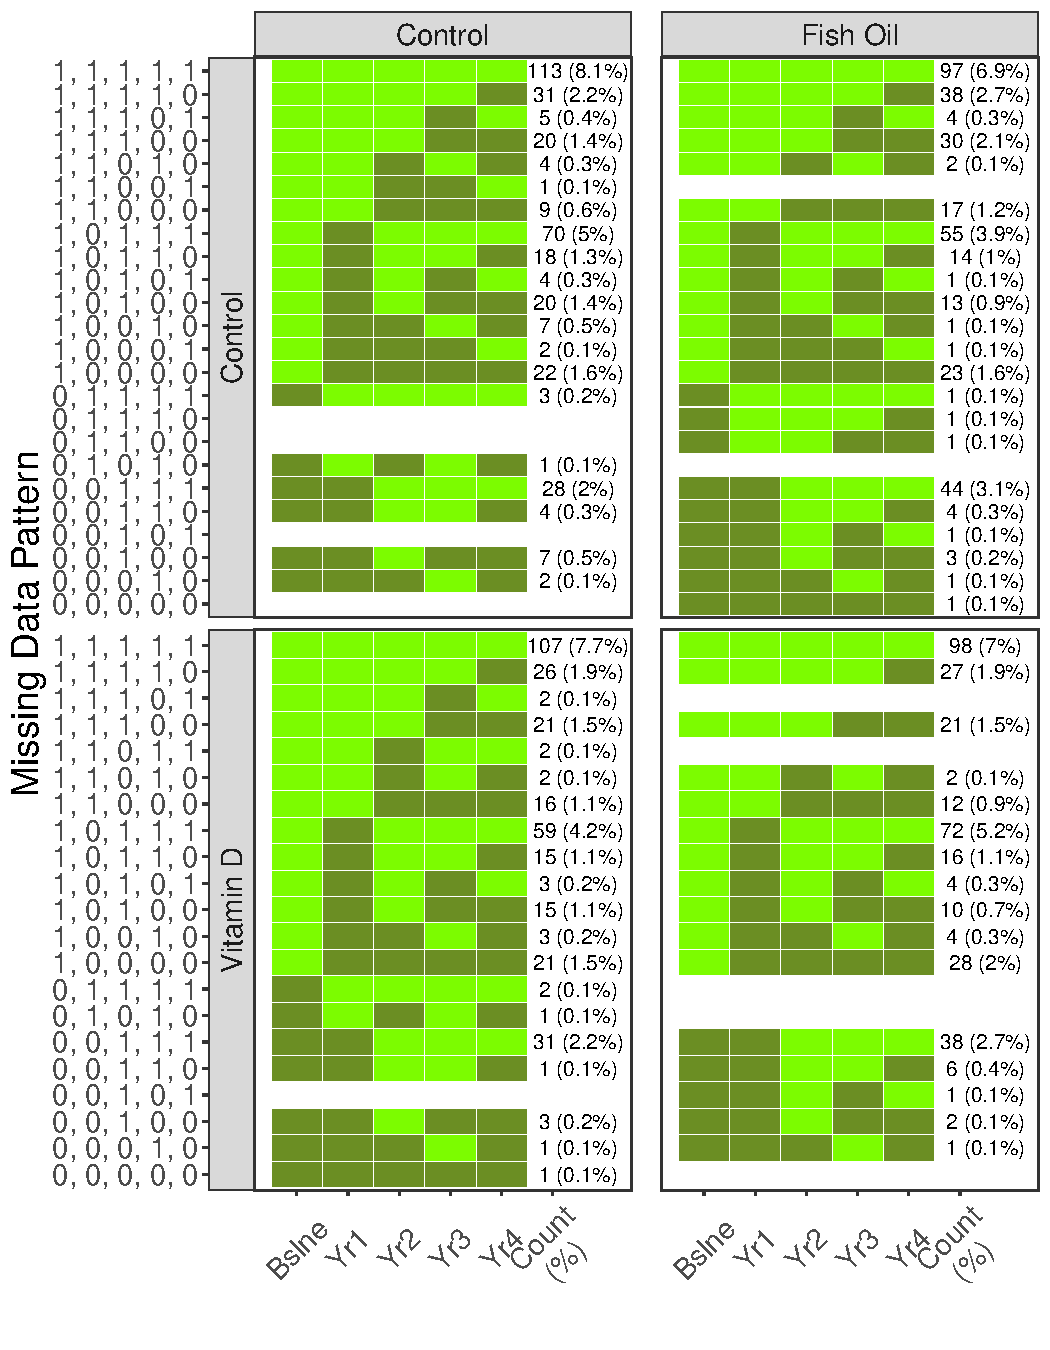
\includegraphics[keepaspectratio]{Final_Report_files/figure-latex/unnamed-chunk-23-1.pdf}}

Figure 2.x: Higher percentage of missing data in control group

If we investigate the missing data pattern in more detail, we can see
that the pattern is similar in both groups. In the plot below, we can
see that the pattern in which the three headache severity scores
\(pk1\), \(pk2\) and \(pk5\) are observed (1,1,1) followed by the
pattern in which both post-randomised headache severity scores contain
missing data (1,0,0).

\pandocbounded{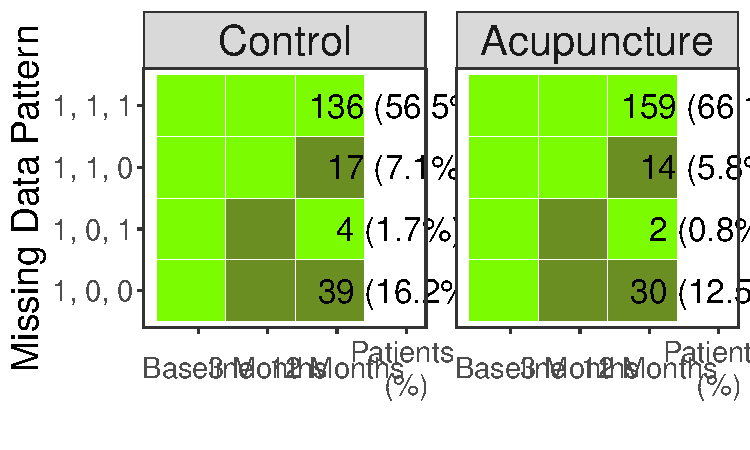
\includegraphics[keepaspectratio]{Final_Report_files/figure-latex/unnamed-chunk-24-1.pdf}}

Figure 2.x: Missing data pattern is similar in both groups (1=observed,
0=missing)

\textbf{VITAL data}

The summary statistics of the VITAL data showed, unlike the acupuncture
trial data, there are also baseline variables that contain missing data
as well as the post randomised variables. A non-monotic multivariate
pattern appears to show here as there is a great proportion of missing
data in the knee pain score at the first year post randomisation, which
drastically decreases in year 2, then steadily increases again.

\pandocbounded{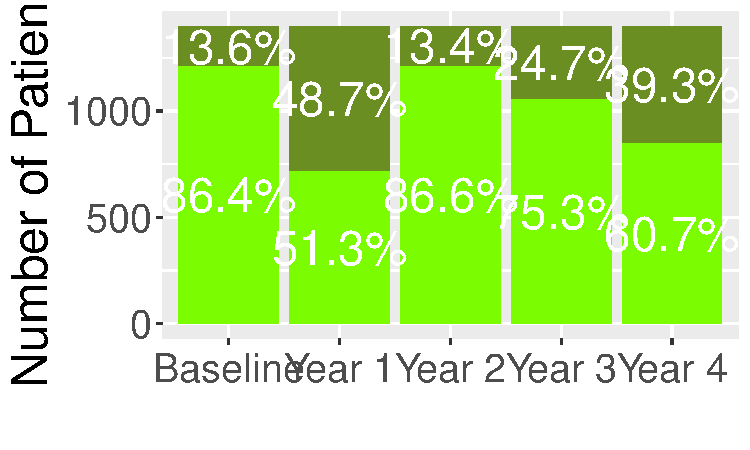
\includegraphics[keepaspectratio]{Final_Report_files/figure-latex/unnamed-chunk-25-1.pdf}}

Figure 2.x: Non-monotonic pattern across out knee pain scores in VITAL
data.

Recall that the VITAL data set contains 4 different combinations of
treatment. Separating this out in the plot below we can see the
percentage of missing data in each knee pain time point variable in each
group. The proportion appears to be similar in each group with year 2
post randomisation containing the most missing data.

\pandocbounded{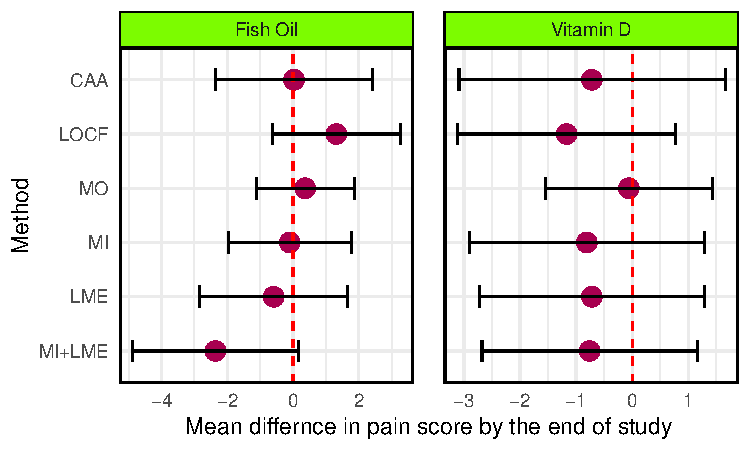
\includegraphics[keepaspectratio]{Final_Report_files/figure-latex/unnamed-chunk-26-1.pdf}}

Figure 2.x: Percentage of missing data across baseline and 4 follow-up
time points. Non-monotonic pattern appears similar in 4 randomised
groups.

Looking at the possible missing data patterns in the 4 combinatory
groups, they are mostly similar with little anomalies. As this dataset
has more time-points recorded than the acupuncture trial data, and more
treatmenr groups, there are more possible missing data patterns to
observe. The most common data pattern still stands as (1,1,1,1,1) in
which data is observed at all time-points.

\pandocbounded{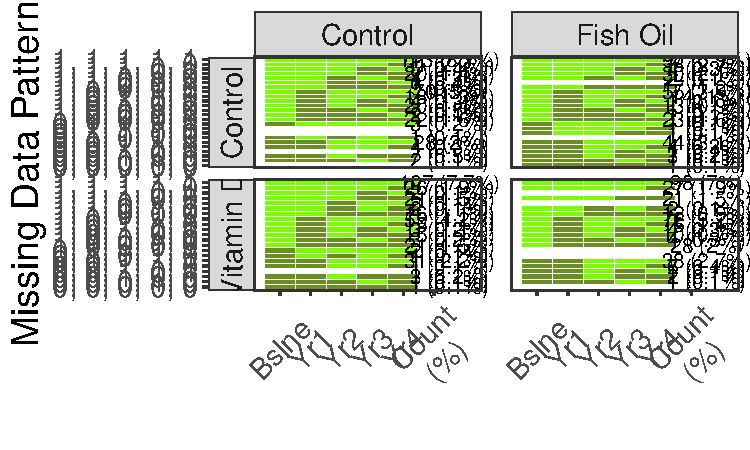
\includegraphics[keepaspectratio]{Final_Report_files/figure-latex/unnamed-chunk-27-1.pdf}}

Figure 2.x: Missing data patterns across 4 treatment groups in VITAL
data.

\newpage

\section{Methods}\label{methods}

\subsection{Data wrangling}\label{data-wrangling}

The VITAL dataset was originally in wide format, which is not suitable
for methods like linear mixed-effects models (LME) that require
long-format data. To address this, the data was reshaped to long format
using pivot\_longer(), as illustrated in the example code provided for
VITAL.

\begin{Shaded}
\begin{Highlighting}[]
\CommentTok{\# Function for transform}
\NormalTok{to\_long\_format\_vital }\OtherTok{\textless{}{-}} \ControlFlowTok{function}\NormalTok{(data\_wide) \{}
\NormalTok{  data\_wide }\SpecialCharTok{\%\textgreater{}\%}
    \FunctionTok{pivot\_longer}\NormalTok{(}\AttributeTok{cols =} \FunctionTok{matches}\NormalTok{(}\StringTok{"\_yr[[:digit:]]$"}\NormalTok{),}
                 \AttributeTok{names\_to =} \FunctionTok{c}\NormalTok{(}\StringTok{".value"}\NormalTok{, }\StringTok{"time"}\NormalTok{), }
                 \AttributeTok{names\_sep =} \StringTok{"\_"}\NormalTok{) }\SpecialCharTok{\%\textgreater{}\%}
    \FunctionTok{mutate}\NormalTok{(}\AttributeTok{time\_contin =} \FunctionTok{as.integer}\NormalTok{(}\FunctionTok{gsub}\NormalTok{(}\StringTok{"yr"}\NormalTok{, }\StringTok{""}\NormalTok{, time)),}
           \AttributeTok{time\_contin\_cent =}\NormalTok{ time\_contin }\SpecialCharTok{{-}} \DecValTok{4}\NormalTok{)}
\NormalTok{\}}
\CommentTok{\# Apply function}
\NormalTok{vital\_long }\OtherTok{\textless{}{-}} \FunctionTok{to\_long\_format\_vital}\NormalTok{(vital\_wide)}
\end{Highlighting}
\end{Shaded}

In the case of multiple imputation (MI), imputation was first performed
on the wide-format data using the mice() function. The resulting imputed
datasets were then combined and transformed to long format, allowing for
the inclusion of time as a continuous variable. This approach enables
the application of LME as the substantive model, which effectively
accounts for repeated measurements over time. Moreover, it accommodates
more flexible timing of follow-up assessments. An example code snippet
demonstrates how the acupunture imputed dataset was processed and
analyzed using this method.

\begin{Shaded}
\begin{Highlighting}[]
\CommentTok{\# Multi{-}imputation in wide format data}
\NormalTok{acu\_mice }\OtherTok{\textless{}{-}} \FunctionTok{mice}\NormalTok{(acu\_wide, }\AttributeTok{m =} \DecValTok{5}\NormalTok{, }\AttributeTok{method =} \StringTok{\textquotesingle{}pmm\textquotesingle{}}\NormalTok{, }\AttributeTok{seed =} \DecValTok{123}\NormalTok{, }\AttributeTok{print=}\ConstantTok{FALSE}\NormalTok{)}
\CommentTok{\# Stack 5 imputations together}
\NormalTok{acu\_mice\_data\_wide }\OtherTok{\textless{}{-}} \FunctionTok{complete}\NormalTok{(}\AttributeTok{data =}\NormalTok{ acu\_mice, }\AttributeTok{action =} \StringTok{"long"}\NormalTok{, }\AttributeTok{include =} \ConstantTok{TRUE}\NormalTok{)}
\CommentTok{\# Function to transform wide imputed data to long}
\NormalTok{to\_long\_format\_acu\_cat\_MICE }\OtherTok{\textless{}{-}} \ControlFlowTok{function}\NormalTok{(data\_wide) \{}
\NormalTok{  data\_wide }\SpecialCharTok{\%\textgreater{}\%}
    \FunctionTok{pivot\_longer}\NormalTok{(}
      \AttributeTok{cols =} \FunctionTok{c}\NormalTok{(}\StringTok{\textquotesingle{}pk2\textquotesingle{}}\NormalTok{, }\StringTok{\textquotesingle{}pk5\textquotesingle{}}\NormalTok{), }
      \AttributeTok{names\_to =} \StringTok{\textquotesingle{}pk\_time\textquotesingle{}}\NormalTok{,}
      \AttributeTok{values\_to =} \StringTok{\textquotesingle{}pk\_score\textquotesingle{}}
\NormalTok{    ) }\SpecialCharTok{\%\textgreater{}\%}
    \FunctionTok{pivot\_longer}\NormalTok{(}
      \AttributeTok{cols =} \FunctionTok{c}\NormalTok{(}\StringTok{\textquotesingle{}f2\textquotesingle{}}\NormalTok{, }\StringTok{\textquotesingle{}f5\textquotesingle{}}\NormalTok{), }
      \AttributeTok{names\_to =} \StringTok{\textquotesingle{}freq\_time\textquotesingle{}}\NormalTok{,}
      \AttributeTok{values\_to =} \StringTok{\textquotesingle{}freq\_score\textquotesingle{}}\NormalTok{,}
      \AttributeTok{names\_repair =} \StringTok{\textquotesingle{}unique\textquotesingle{}}
\NormalTok{    ) }\SpecialCharTok{\%\textgreater{}\%}
    \FunctionTok{filter}\NormalTok{((pk\_time }\SpecialCharTok{==} \StringTok{\textquotesingle{}pk2\textquotesingle{}} \SpecialCharTok{\&}\NormalTok{ freq\_time }\SpecialCharTok{==} \StringTok{\textquotesingle{}f2\textquotesingle{}}\NormalTok{) }\SpecialCharTok{|}\NormalTok{ (pk\_time }\SpecialCharTok{==} \StringTok{\textquotesingle{}pk5\textquotesingle{}} \SpecialCharTok{\&}\NormalTok{ freq\_time }\SpecialCharTok{==} \StringTok{\textquotesingle{}f5\textquotesingle{}}\NormalTok{)) }\SpecialCharTok{\%\textgreater{}\%}
    \FunctionTok{mutate}\NormalTok{(}
      \AttributeTok{time =} \FunctionTok{case\_when}\NormalTok{(}
\NormalTok{        pk\_time }\SpecialCharTok{==} \StringTok{\textquotesingle{}pk2\textquotesingle{}} \SpecialCharTok{\textasciitilde{}} \StringTok{"3m"}\NormalTok{,}
\NormalTok{        pk\_time }\SpecialCharTok{==} \StringTok{\textquotesingle{}pk5\textquotesingle{}} \SpecialCharTok{\textasciitilde{}} \StringTok{"12m"}
\NormalTok{      )}
\NormalTok{    ) }\SpecialCharTok{\%\textgreater{}\%}
    \FunctionTok{select}\NormalTok{(}\SpecialCharTok{{-}}\NormalTok{pk\_time, }\SpecialCharTok{{-}}\NormalTok{freq\_time) }\SpecialCharTok{\%\textgreater{}\%}
    \FunctionTok{group\_by}\NormalTok{(.imp) }\SpecialCharTok{\%\textgreater{}\%}
    \FunctionTok{mutate}\NormalTok{(}\AttributeTok{.id =} \FunctionTok{row\_number}\NormalTok{())}
\NormalTok{\}}
\CommentTok{\# Apply function}
\NormalTok{acu\_mice\_data\_long }\OtherTok{\textless{}{-}} \FunctionTok{to\_long\_format\_acu\_cat\_MICE}\NormalTok{(acu\_mice\_data\_wide)}
\CommentTok{\# Transform object to mid}
\NormalTok{acu\_mice\_data\_obj\_long }\OtherTok{\textless{}{-}} \FunctionTok{as.mids}\NormalTok{(acu\_mice\_data\_long)}
\CommentTok{\# Apply LME as substantive model}
\NormalTok{acu\_LME\_MI\_default }\OtherTok{\textless{}{-}} \FunctionTok{with}\NormalTok{(acu\_mice\_data\_obj\_long, }
                           \FunctionTok{lmer}\NormalTok{(pk\_score }\SpecialCharTok{\textasciitilde{}}\NormalTok{ group}\SpecialCharTok{*}\NormalTok{time }\SpecialCharTok{+}\NormalTok{ pk1 }\SpecialCharTok{+}\NormalTok{ (}\DecValTok{1}\SpecialCharTok{|}\NormalTok{id)))}
\CommentTok{\# Pool for parameter estimation}
\NormalTok{acu\_LME\_MI\_default\_pool }\OtherTok{\textless{}{-}} \FunctionTok{pool}\NormalTok{(acu\_LME\_MI\_default)}
\end{Highlighting}
\end{Shaded}

\subsection{Anchoring methods}\label{anchoring-methods}

We began our analysis with basic methods to serve as a comparison
benchmark for more advanced techniques. As previously mentioned, these
included complete case analysis, last observation carried forward
(LOCF), and the mean observation method. Each of these approaches was
used to anchor the results and provide a reference point for evaluating
the performance of more robust models.

\subsubsection{Complete case analysis}\label{complete-case-analysis}

For both data sets, given that our estimand is the mean difference in
pain scores at the end of the study, we fit a model regressing the final
pain score on treatment group and baseline pain score. If the data are
Missing Completely At Random (MCAR), complete case analysis (CCA) can
yield valid inference. For simplicity and to conserve computational
resources, we did not adjust for additional baseline covariates. To
maintain comparability across methods, we omit these covariates in the
other analyses as well.

We applied the following models for each dataset:

\begin{Shaded}
\begin{Highlighting}[]
\CommentTok{\# For acupuncture data set}
\NormalTok{acu\_CAA }\OtherTok{\textless{}{-}} \FunctionTok{lm}\NormalTok{(pk5 }\SpecialCharTok{\textasciitilde{}}\NormalTok{ group }\SpecialCharTok{+}\NormalTok{ pk1 , }\AttributeTok{data =}\NormalTok{ acu\_wide)}
\CommentTok{\# For VITAL data set}
\NormalTok{vital\_complete }\OtherTok{\textless{}{-}} \FunctionTok{lm}\NormalTok{(pain\_yr4 }\SpecialCharTok{\textasciitilde{}}\NormalTok{ fishoilactive }\SpecialCharTok{+}\NormalTok{ vitdactive }\SpecialCharTok{+}\NormalTok{ pain\_base, }\AttributeTok{data =}\NormalTok{ vital\_wide)}
\end{Highlighting}
\end{Shaded}

One of the main drawbacks of using complete case analysis (CCA) is the
loss of power due to reduced sample size, along with the risk of
introducing bias. In our implementation, the lm() function in R
automatically excludes any individual with missing values in the model
variables. As a result, we are left with only 301 out of 401
observations in the acupuncture dataset and 698 out of 1390 in the VITAL
dataset---corresponding to a loss of approximately 25\% and 50\% of the
sample size, respectively.

Although both datasets are relatively large, the reduction in
statistical power from complete case analysis may be less of a concern.
However, the potential for bias remains a more serious issue. We have
not included many covariates in our models, so bias could exist even
with complete data due to omitted variables. Now, suppose we attempted
to adjust for all relevant baseline covariates---missing data would
still pose a problem. For instance, in the VITAL dataset, several
baseline covariates have missing values. Excluding observations with
missing data in these variables could still induce bias, considering the
missingness could be related to the outcome.

In the acupuncture dataset, although there is no missingness in baseline
variables, complete case analysis still has two major limitations.
First, it does not allow for adjustment of interim outcomes, such as the
3-month pain score. This limitation can be addressed by using a linear
mixed-effects model, which accounts for repeated measurements over time.
Second, auxiliary variables---such as pain frequency---cannot be
included in this model, even though they may help improve estimation.
This issue can be resolved through multiple imputation, which allows the
use of additional information to handle missing data more effectively.

In rare cases---such as when the sole interest is in estimating the mean
difference between groups at the end of the study, and there are no
important non-baseline covariates complete case analysis can still yield
valid results. Thus when apply complete case analysis, we are assuming:
the outcome is Missing At Random (MAR), conditional on the observed
baseline predictors included in the model.

This condition sometimes referred to as ``conditionally MCAR''. While it
is weaker than the strict MCAR assumption, it is still quite strong. It
implies that:

\begin{itemize}
\tightlist
\item
  Missingness depends only on the variables included in the model;
\item
  The model is correctly specified;
\item
  The outcome variable is not involved in the missingness
  mechanism---consistent with the MAR framework.
\end{itemize}

Under these assumptions, CCA can provide unbiased estimates. However,
they are rarely fully met in practice, especially in complex
longitudinal studies where many relevant variables and time points are
involved.

This can be expressed in the mathematics form, assuming outcome of
interest Y MAR depends on baseline covaraites X

\begin{align*}
  Pr(Ri=r \mid Yi, Xi) = Pr(Ri=r \mid Xi)
  \end{align*}

Thus, we can infer under MAR, the distribution of outcome within
covaraites is the same in the observed data, the unobserved data, and
the population.

\begin{align*}
  & Pr(Yi \mid Ri=r, Xi) \\ 
  & = \displaystyle \frac{Pr(Ri=r,Yi,Xi)}{Pr(Ri=r,Xi)} \\
  & = \displaystyle \frac{Pr(Ri=r \mid Yi,Xi)Pr(Yi,Xi)}{Pr(Ri=r \mid Xi)Pr(Xi)} 
  \\
  & Assuming \ \ \Pr(Ri=r \mid Yi, Xi) = Pr(Ri=r \mid Xi) \\
  & = \displaystyle \frac{Pr(Yi,Xi)}{Pr(Xi)} \\
  & = Pr(Yi \mid Xi)
  \end{align*}

The key issue is that we aim to include as much relevant information as
possible in the set of predictors X to make the MAR assumption more
plausible and robust. As discussed above, more statistically principled
methods---such as multiple imputation or mixed-effects models---allow us
to incorporate a broader set of variables and handle missingness more
effectively. However, it is important to note that the MAR assumption is
fundamentally untestable. Therefore, to assess the robustness of our
conclusions, we must perform sensitivity analyses, which are presented
in later sections.

\subsubsection{Last observation carry
forward}\label{last-observation-carry-forward}

Last Observation Carried Forward (LOCF) is a simple imputation method
that fills in missing values based on the last observed outcome for each
subject. It relies on assumptions unrelated to the missing data
mechanism, meaning it does not model the reason for missingness.
Instead, LOCF assumes that the outcome remains stable after dropout,
which may be plausible in some clinical contexts, such as when the
treatment effect has plateaued or when patients are expected to remain
in a steady state.

However, this assumption is not convincing in either of the datasets
analyzed here. In both the Acupuncture and VITAL trials, pain score are
unlikely to be stabilized throughout, and the outcomes display trends
over time, making the LOCF assumption potentially misleading and
unsuitable for accurate estimation of treatment effects.

Below is the R code used to perform LOCF imputation on the data in wide
format. Following imputation, we fitted the resulting dataset using the
lm() function, consistent with the approach used in the complete case
analysis (CAA):

\begin{Shaded}
\begin{Highlighting}[]
\CommentTok{\# LOCF function}
\NormalTok{LOCF }\OtherTok{\textless{}{-}} \ControlFlowTok{function}\NormalTok{(data, columns)\{}
  \ControlFlowTok{for}\NormalTok{ (col }\ControlFlowTok{in}\NormalTok{ columns) \{}
    \ControlFlowTok{for}\NormalTok{ (i }\ControlFlowTok{in} \DecValTok{1}\SpecialCharTok{:}\FunctionTok{nrow}\NormalTok{(data)) \{  }
      \ControlFlowTok{if}\NormalTok{ (}\FunctionTok{is.na}\NormalTok{(data[i, col])) \{}
\NormalTok{        data[i, col] }\OtherTok{\textless{}{-}}\NormalTok{ data[i, col }\SpecialCharTok{{-}} \DecValTok{1}\NormalTok{]  }
\NormalTok{      \}}
\NormalTok{    \}}
\NormalTok{  \}}
  \FunctionTok{return}\NormalTok{(data)  }
\NormalTok{\}}
\end{Highlighting}
\end{Shaded}

\subsubsection{Mean observation method}\label{mean-observation-method}

Mean imputation is another simple method that fills in missing values by
replacing them with the mean of the observed data at each timepoint.
Like LOCF, it is based on assumptions unrelated to the missing data
mechanism and does not attempt to model why the data are missing.

This method implicitly assumes that the mean of the observed values
accurately represents the population mean, which can be problematic. In
fact, this can be viewed as an even more radical assumption than
assuming data are Missing Completely At Random (MCAR), since it ignores
potential bias introduced by the missingness and oversimplifies
individual variation.

As with LOCF, this assumption is not convincing in either of the
datasets analyzed here. In both the Acupuncture and VITAL trials, pain
scores vary over time, and individual trajectories differ. Replacing
missing values with the average observed value at each timepoint
disregards this variation and may lead to underestimated variability and
biased treatment effect estimates.

Below is the R code used to perform mean imputation on the data in wide
format. Following imputation, we fitted the resulting dataset using the
lm() function, as in the complete case analysis (CAA):

\begin{Shaded}
\begin{Highlighting}[]
\NormalTok{mean\_impute }\OtherTok{\textless{}{-}} \ControlFlowTok{function}\NormalTok{(data) \{}
\NormalTok{  data }\OtherTok{\textless{}{-}} \FunctionTok{data.frame}\NormalTok{(}
    \FunctionTok{lapply}\NormalTok{(data, }\ControlFlowTok{function}\NormalTok{(x) \{}
      \ControlFlowTok{if}\NormalTok{ (}\FunctionTok{is.numeric}\NormalTok{(x)) \{}
        \FunctionTok{return}\NormalTok{(}\FunctionTok{ifelse}\NormalTok{(}\FunctionTok{is.na}\NormalTok{(x), }\FunctionTok{mean}\NormalTok{(x, }\AttributeTok{na.rm =} \ConstantTok{TRUE}\NormalTok{), x))}
\NormalTok{      \} }\ControlFlowTok{else}\NormalTok{ \{}
        \FunctionTok{return}\NormalTok{(x)}
\NormalTok{      \}}
\NormalTok{    \})}
\NormalTok{  )}
  \FunctionTok{return}\NormalTok{(data)}
\NormalTok{\}}
\end{Highlighting}
\end{Shaded}

\subsection{Changing imputation
methods}\label{changing-imputation-methods}

To address missing data in a statistically principled manner, it is
helpful to distinguish between two components: the imputation step and
the modeling step. In our anchoring methods, we either did not perform
imputation---as in complete case analysis (CCA)---or relied on single
imputation techniques, such as last observation carried forward (LOCF)
or mean imputation.

While methods like linear mixed-effects models (LME) can utilize most
available observed data and yield unbiased estimates under the Missing
At Random (MAR) assumption without imputation, they cannot incorporate
auxiliary variables that are not part of the model (e.g., pain frequency
in the Acupuncture dataset). In contrast, multiple imputation (MI)
allows the inclusion of such auxiliary information during the imputation
process.

In most realistic scenarios, doing no imputation or applying single
imputation methods is likely to introduce bias and underestimate
uncertainty, especially when missingness is related to unobserved
outcomes. Thus, more flexible approaches---such as MI combined with
appropriate modeling---are generally preferred for robust inference in
the presence of missing data.

\subsubsection{Multiple imputation}\label{multiple-imputation}

A key limitation of single imputation methods is that they treat imputed
values as if they were observed data when fitting the substantive model.
This approach fails to reflect the inherent uncertainty associated with
missing values---it assumes we have perfectly recovered the unobserved
data, which is never the case in practice.

In reality, the best we can do is to estimate the distribution of the
missing data conditional on the observed data, under specific
assumptions about the missingness mechanism (e.g., MAR). Importantly,
this distribution is not adequately captured by a single draw, as is
done in single imputation. Instead, to account for uncertainty, we must
generate multiple draws from this distribution, resulting in multiple
imputed datasets. This is the foundation of Multiple Imputation (MI).

As we will demonstrate in the following sections, the draws used in MI
must be (at least approximately) Bayesian for Rubin's variance formula
to yield valid inference. By fitting the substantive model separately to
each of the K completed datasets, we obtain multiple estimates that,
when pooled, incorporate both within-imputation variability and
between-imputation variability. This approach not only addresses bias
caused by missing data but also appropriately inflates standard errors
to reflect the uncertainty introduced by imputation. Rubin's rules
provide a general framework for combining these estimates to obtain
point estimates, variances, confidence intervals, and statistical tests.

We also briefly introduce the different methods available for performing
multiple imputation. In cases with a monotonic missing data pattern,
sequential regression offers a straightforward solution. For arbitrary
or multivariate missingness, more flexible approaches like joint
modeling or Fully Conditional Specification (FCS)---also known as
multiple imputation by chained equations (MICE)---are required.

In our project, we chose the FCS approach, given its flexibility and
ease of use when dealing with datasets like Acupuncture and VITAL that
have complex missingness patterns across multiple variables. A brief
comparison of joint modeling versus FCS is included below to justify
this decision.

While we used five imputations (K = 5) for our MI procedure in this
analysis, we also discuss the considerations involved in choosing the
number of imputations. These include factors such as the proportion of
missing data, computational cost, and the desired precision of standard
errors and confidence intervals.

\paragraph{Rubin's rules}\label{rubins-rules}

Once multiple imputed datasets are generated, Rubin's rules are used to
combine the parameter estimates and associated uncertainty across the K
imputed datasets. The steps are as follows:

\begin{enumerate}
\def\labelenumi{\arabic{enumi}.}
\item
  Impute K complete datasets, each containing different plausible values
  for the missing data. (More details in later section, we will focus on
  the following steps for now)
\item
  Fit the substantive model (e.g., a linear model or mixed-effects
  model) to each imputed dataset, obtaining Parameter estimate
  \(\hat{\beta}_{k}\) and Variance estimate \(\hat{\sigma}_{k}^{2}\) for
  each k=1,2,\ldots,K
\item
  Compute the pooled estimate \(\hat{\beta}_{MI}\) and its total
  variance \(\hat{V}_{MI}\): \begin{align*}
    \hat{\beta}_{MI} = \frac{1}{K} \sum_{k=1}^{K}{\hat{\beta}_{k}} \\
    \hat{V}_{MI} = \hat{W} + (1 + \frac{1}{K}) \hat{B} \\
    \hat{W} = \frac{1}{K} \sum^{K}_{k=1}{\hat{\sigma}^{2}_{k}} \\
    \hat{B} = \frac{1}{K-1} \sum^{K}_{k=1}({\hat{\beta}_{k}} - \hat{\beta_{MI}})^{2} \\
    \end{align*}
\item
  To test a null hypothesis \(\hat{\beta}_{MI} = \beta^{0}\) use a
  t-statistic with \(\nu\) degrees of freedom. This allows us to
  construct confidence intervals and perform hypothesis testing,
  reflecting the additional uncertainty due to imputation.
  \begin{align*}
    T = \frac{\hat{\beta}_{MI} - \beta^{0}}  {\sqrt{\hat{V}_{MI}}} \\
    \nu = (K-1)[1 + \frac{\hat{W}}{(1 + 1/K) \hat{B}}]^{2}
    \end{align*}
\end{enumerate}

\paragraph{Sequential regression MI}\label{sequential-regression-mi}

In many longitudinal studies, the missing data pattern is approximately
monotonic, particularly when dropout is due to participant withdrawal, a
common situation in clinical research. In such cases, later measurements
are often missing while earlier ones are observed, which permits the use
of sequential regression for imputation under the assumption of Missing
At Random (MAR).

To justify this, consider the joint distribution of the outcome vector
for individual \(i\) can be factorized as:

\begin{align*}
    f(Y_{i,1},Y_{i,2},...,Y_{i,p}) = f(Y_{i,p} \mid Y_{i,1},...,Y_{i,p-1}) * 
    f(Y_{i,p-1} \mid Y_{i,1},...,Y_{i,p-2}) * ... * f(Y_{i,2} \mid Y_{i,1}) 
    * f(Y_{i,1})
    \end{align*}

Under a monotonic missingness pattern, for each missing value
\(Y_{i,j}\) all preceding values \(Y_{i,1},...,Y_{i,j-1}\) are observed.
If we also assume Missing At Random (MAR), then each of these
conditional distributions can be estimated directly from the observed
data. This provides a principled basis for sequential regression
imputation, where each variable is regressed on the variables preceding
it in order, and missing values are imputed based on those conditional
models.

Suppose we have \(i=1,...,n\) individual with \(j=1,...,p\) variables.
When the missing data pattern is monotonic, sequential regression
provides an efficient and valid approach to imputation under the MAR
assumption. The procedure follows these steps:

\begin{enumerate}
\def\labelenumi{\arabic{enumi}.}
\tightlist
\item
  specify the model
\end{enumerate}

\begin{align*}    
    Y_{i,j} = (1,Y_{i,1},...,Y_{i,j-1})^{T} * \beta_{j} + 
    e_{i,j},\ {e_{i,j}^{i.i.d.} \sim{N} (0,\sigma^{2}_{j})}
    \end{align*}

\begin{enumerate}
\def\labelenumi{\arabic{enumi}.}
\setcounter{enumi}{1}
\item
  Under the monotonic pattern, for every missing \(Y_{i,j}\) we assume
  that \(Y_{i,1},...,Y_{i,j-1}\) are fully observed. We fit the
  regression model using ordinary least squares (OLS) to obtain
  estimates \(\hat{\beta}_{j},\hat{\sigma}_{j}^{2}\)
\item
  To incorporate uncertainty, we draw new parameters
  \(\beta_{j}^{*},\sigma_{j}^{*2}\) from their posterior distributions:
\end{enumerate}

\begin{align*}
   \sigma_j^{*2} = \frac{\hat{\sigma}_j^2 (n_j - j)}{z} \\
   \beta^* \sim N(\hat{\beta}, \sigma_j^{*2} A_j) \\
   A_j = (\sum_{i=1}^{n_j} x_{i,j} x_{i,j}^T)^{-1}
   \end{align*}

\begin{enumerate}
\def\labelenumi{\arabic{enumi}.}
\setcounter{enumi}{3}
\item
  For individuals with missing \(Y_{i,j}\) generate imputations from the
  model:
  \(Y_{i,j} = (1,Y_{i,1},...,Y_{i,j-1}) \beta^{*} + e^{*}_{i,j}\),
  \(e_{i,j}^{*} \sim{N} (0,\sigma^{*2}_{j})\)
\item
  Repeat for \(Y_{i,j+1}\) until complete
\end{enumerate}

This sequential regression method is applicable to datasets with a
monotonic missingness pattern, such as the Acupuncture dataset, where
individuals tend to drop out in a consistent, time-ordered manner.
However, it is not suitable for datasets with non-monotonic missingness,
such as VITAL, where some individuals may have missing values at
intermediate time points but return for later follow-ups. In such cases,
more flexible approaches like Joint Modeling or Fully Conditional
Specification (FCS) are required to properly handle the complex,
arbitrary missing data structure.

\paragraph{Joint modelling}\label{joint-modelling}

When the missing data pattern is non-monotonic, as in the VITAL dataset,
sequential regression is no longer appropriate. Instead, we can apply
joint modeling, which makes no assumption about the missingness pattern
but assumes the missing data mechanism is ignorable (typically, Missing
At Random).

Under joint modeling, we assume that the complete multivariate outcome
vector follows a multivariate normal distribution: \begin{align*}
    & Y \sim N(\beta,\ \Omega) \\
    & Y = (Y_{i,1},Y_{i,2},...,Y_{i,p})^{T} \\
    & \beta = (\beta_{0,1},\beta_{0,2},...,\beta_{0,p})^{T} \\
    & \Omega \ \text{is the covariance matrix}
    \end{align*}

To estimate the parameters \(\beta\) and \(\Omega\) and impute missing
values, Gibbs sampling is one of the approaches. This algorithm draws
each parameter in turn, conditional on the current values of all other
parameters and the data.

To get priors to start Gibbs sampling. We begin with initial estimates
\(\beta^{0}\) and \(\Omega^{0}\), computed from the observed data. For
each variable with missing values, we also generate an initial
imputation \(Y_{M}^{0}\) by sampling from the observed values of that
variable with replacement. This allows us to calculate initial
statistics such as \(\overline{Y}^{0}\) and and the sample covariance
matrix \(S^{0}\) (Note it also used as prior sample covariance matrix
\(S^{P}\) in each iteration)

Then, for each iteration r the following steps are performed:

\begin{enumerate}
\def\labelenumi{\arabic{enumi}.}
\item
  Draw the precision matrix (inverse
  covariance):\(\Omega^{-1,r} \sim W(n + \nu, (S_p^{-1} + S^{r-1})^{-1})\)
\item
  Draw the mean
  vector:\(\beta^{r} \sim N(\bar{Y}^{r-1}, n^{-1} \Omega^r)\)
\item
  Impute missing values:
  \(Y_{M}^{r} \sim f(Y_{M} \mid \beta^{r}, \Omega^{r}, Y_{O})\)
\item
  Update the mean and covariance estimates: \(\bar{Y}^{r}\) the mean of
  the combined imputed and observed data, and \(S^{r}\) the sum of
  squares and cross-products from the combined data
\end{enumerate}

After a sufficient number of burn-in iterations, we repeat this process
K times to generate K imputed datasets. These are then analyzed using
the substantive model of interest, and Rubin's rules are applied to pool
the results, yielding valid parameter estimates and standard errors that
account for the uncertainty due to missing data.

\paragraph{Full conditional
specification}\label{full-conditional-specification}

Fully Conditional Specification (FCS), also known as multiple imputation
by chained equations (MICE), is an extension of sequential regression
imputation that relaxes the requirement that all covariate values used
in the regressions be fully observed.

Importantly, when the missingness pattern is monotonic, FCS becomes
equivalent to the sequential regression method discussed earlier.
However, its key advantage is that it remains valid under non-monotonic
missingness, making it suitable for more general data structures like
the VITAL dataset.

The term ``full conditional specification'' refers to the fact that each
variable is imputed from its full conditional distribution, given all
other variables. This allows for more flexible modeling of multivariate
missingness.

The general procedure involves the following steps:

\begin{enumerate}
\def\labelenumi{\arabic{enumi}.}
\item
  Reorder the variables so that the overall missingness pattern is as
  close to monotonic as possible. This can improve stability and
  convergence in the imputation process.
\item
  Initialize missing values by filling in initial guesses---often by
  drawing, with replacement, from the observed values of each variable.
\item
  For each variable \(Y_{j}\)

  \begin{itemize}
  \tightlist
  \item
    Regress the observed part of \(Y_{j}\) on all other variables
    (including those with imputed values).
  \item
    Use the fitted model to impute the missing values in \(Y_{j}\),
    treating the other variables as given.
  \end{itemize}
\item
  Repeat step 3 for all variables with missing data to complete one
  cycle.
\item
  Perform multiple cycles until convergence, and then repeat the entire
  process K times to generate K imputed datasets.
\end{enumerate}

These datasets can then be analyzed with the substantive model, and the
results pooled using Rubin's rules. FCS is widely used in practice due
to its flexibility and implementation in tools like the mice package in
R.

\paragraph{FCS VS joint modelling}\label{fcs-vs-joint-modelling}

Generally, under the assumption of a multivariate normal distribution,
the joint distribution uniquely determines the full set of conditional
distributions, and vice versa. This means that, in theory, joint
modeling and fully conditional specification (FCS) are mathematically
compatible representations of the same underlying structure---provided
all models are correctly specified.

In practice, however, joint modeling using a Gibbs sampler is often
considered a more efficient algorithm. It also has the advantage of
allowing the inclusion of prior information, which can be particularly
useful when data are sparse or when integrating external knowledge into
the model. Additionally, joint modeling methods can incorporate ridge
parameters to stabilize the estimation of the covariance matrix, which
becomes important when the number of variables is large relative to the
sample size.

However, these concerns do not apply in our project, as our datasets
have moderate dimensionality and sufficient sample size. Therefore, we
opted to use Fully Conditional Specification (FCS) for multiple
imputation.

FCS is also easier to implement, since it does not require explicit
specification of a joint model or priors, and it generally requires
fewer iterations to reach convergence in practical settings. For these
reasons, we adopted the FCS approach using the mice package in R to
perform multiple imputation throughout this project.

Finally, within the MICE framework, different imputation methods can be
specified for different variable types---such as predictive mean
matching or sampling from observed values. We will explore the impact of
these options later in the analysis.

\paragraph{How to choose m}\label{how-to-choose-m}

Another practical consideration in multiple imputation (MI) is the
choice of the number of imputations, denoted by K. While early
applications often used K=5, more recent work emphasizes that the
optimal number depends on the degree of missing information in the data.

A key parameter in determiningK is \(\gamma_{0}\), which represents the
fraction of missing information for the parameter of interest.
Unfortunately, \(\gamma_{0}\) is typically unknown in advance, including
in our project.

To address this, Bodner (2008) proposed a simple and conservative
strategy: using the proportion of complete cases in the dataset as a
proxy for \(1-\gamma_{0}\), thereby estimating \(\gamma_{0}\)
conservatively. This approach allows for an informed yet practical
choice of K, especially when precise calculation of the missing
information is not feasible.

In our analysis, we used K=5 imputations as a baseline, while
recognizing that more imputations may be needed in cases with higher
levels of missingness or if more precise estimates of standard errors
are required. We will explore the implication of changing K in the
following sessions.

\textbf{Choose 3-5 imputations}

The classic advice for multiple imputation is to use a low number of
imputations, typically between 3 and 5, when the proportion of missing
information is moderate. As discussed in Rubin (1987), the argument for
choosing a small K is based on the total variance
estimate:\(T_{K} = (1 + \frac{\gamma0}{K}) T_{\infty}\)

where \(T_{K}\) is the variance with K imputations, \(T_{\infty}\) is
the asymptotic variance as \(K \rightarrow \infty\) and \(\gamma_{0}\)
is the fraction of missing information. Since \(\gamma_{0}\) is
typically unknown, this formula helps illustrate the trade-off between
the number of imputations and efficiency.

There is often limited benefit in increasing K beyond 5. For instance,
if \(\gamma0=30\%\), using K = 5 result in \(T_m=1.06T_\infty\),
indicating only a 6\% inflation in variance compared to the ideal case.

In this project, we chose to use K=5 imputations for multiple
imputation, following the classical recommendation to use a low number
of imputations when the proportion of missing information is moderate.

\textbf{Chosse \textgreater20 imputations}

While early guidelines recommended using a low number of imputations
(typically K=3-5) for moderate missingness, more recent research argue
that increasing K beyond this range can yield important gains in
statistical efficiency.

\begin{itemize}
\tightlist
\item
  Royston (2004) suggested that to constrain the coefficient of
  variation of \(ln(t_{\nu}\sqrt{T})\) to below 0.05---effectively
  keeping the width of confidence intervals within about 10\%
  uncertainty, a minimum of K\textgreater20 is required.
\item
  Graham (2007) argued that to achieve statistical power within 1\% of
  the theoretical maximum, researchers should use at least K=20.
\item
  Bodner (2008) examined how the number of imputations relates to the
  fraction of missing information \(\gamma_{0}\), and its effect on
  p-values and confidence intervals. He recommended increasing
  \(K=(3,6,12,24,59,114,258)\) for \(\gamma0=(0.1, 0.3, 0.5, 0.7, 0.9)\)
  accordingly.
\end{itemize}

In some situations---such as when estimating variance components or when
dealing with highly uncertain estimands---using a very high number of
imputations (e.g.,K=200) may be warranted to approximate the full
posterior distribution.

The main drawback of increasing K is that it leads to longer
computational time. However, this is generally the only limitation, and
it becomes manageable with modern computing resources. Moreover,
starting with a high number of imputations gives greater flexibility: we
can always test the stability or sensitivity of our results by
re-analyzing a subset of the imputations (e.g., comparing the
performance at K=5,10,20) without needing to re-run the entire
imputation process.

Thus, while K=3-5 is often sufficient under moderate missingness and
when the focus is on point estimates, using a larger K can improve
robustness in more demanding settings, with minimal trade-offs beyond
processing time.

\(K \approx 100\lambda\)

A widely cited rule of thumb proposed by White, Royston, and Wood (2011)
recommends choosing the number of imputations based on the fraction of
incomplete cases in the dataset, denoted as \(\lambda\). Specifically,
they suggest setting:\(K \approx 100\lambda\)

This rule has become a de facto standard, particularly in medical
research, due to its simplicity and strong theoretical support. The key
idea is that the number of imputations should roughly match the
percentage of individuals with any missing data.

\begin{itemize}
\item
  The Monte Carlo error of the pooled point estimate \(\hat{\beta}\) is
  approximately 10\% of its standard error.
\item
  The Monte Carlo error of the test statistic
  \(\hat{\beta}/SE_{\hat{\beta}}\) is roughly 0.1.
\item
  The Monte Carlo error of a p-value is approximately 0.01 when the true
  p-value is 0.05.
\end{itemize}

These error bounds are typically acceptable in applied research,
ensuring stable estimates and valid inference without requiring an
excessive number of imputations.

One challenge with applying this rule arises in high-dimensional
settings, where the number of variables is large. In such cases, it is
common for a large proportion of individuals to have at least one
missing value, which can push \(\lambda\) close to 1. To address this,
it is reasonable to use the overall missing rate (i.e., total proportion
of missing cells in the dataset) as a conservative proxy for \(\lambda\)
when needed.

This rule provides a useful upper bound for choosing K, especially when
balancing the goals of statistical precision and computational
efficiency.

\subsection{Changing substantive
model}\label{changing-substantive-model}

Another important decision point in the missing data handling process is
the choice of the substantive model---the model used for the final
analysis after imputation. One natural alternative to standard multiple
linear regression is the linear mixed-effects model (LME).

As discussed earlier, LME has the advantage of leveraging all available
observed data, even in the presence of missingness. In fact, under
certain conditions, LME can yield valid inferences without requiring
multiple imputation, as long as the missingness mechanism is ignorable
(e.g., MAR) and auxiliary variables are not essential.

Moreover, even with fully observed data---either originally complete or
completed through imputation---LME remains a superior choice in many
longitudinal settings because it explicitly accounts for within-subject
correlation from repeated measurements. This leads to more accurate
estimates and better statistical efficiency than standard linear models,
which ignore the data's hierarchical structure.

In this project, we focus on multiple linear regression and LME, both of
which assume a linear relationship between covariates and the outcome.
However, when selecting a substantive model, it's important to evaluate
this assumption. In cases where linearity is questionable, alternative
models---such as polynomial regression or spline-based models---may
provide a better fit and should be considered.

An additional benefit of using LME is that it allows for flexible
modeling of time. Specifically, it enables us to treat time as a
continuous variable, rather than as a categorical factor, which can
improve interpretability and statistical power. This modeling choice
will be explored further in a later section.

\subsection{Examing using forest plot}\label{examing-using-forest-plot}

To visually compare how our estimand (treatment effect) changes across
different missing data methods, we present results using a series of
forest plots. These plots allow us to directly assess the impact of each
imputation or modeling strategy on the estimated effect and its
confidence interval.

The same process was applied to both the Acupuncture and VITAL datasets.
For the VITAL trial, which follows a 2×2 factorial design, we simplify
the analysis---as previously discussed---by treating fish oil and
vitamin D as if they were tested in two separate randomized controlled
trials. This means we ignore potential interaction effects between the
two treatments and estimate their effects independently, which allows
for a more straightforward comparison across methods.

\subsubsection{Change imputation method and substantive
model}\label{change-imputation-method-and-substantive-model}

We evaluated the impact of missing data by systematically varying both
the imputation method and the substantive model used in the analysis. By
doing that, we try to isolate the effects of changing either the
imputation strategy or the analysis model, and highlights the practical
impact of each decision on the resulting treatment effect estimates.

First, as described earlier, we applied three anchoring methods:
Complete Case Analysis (CAA), Last Observation Carried Forward (LOCF),
and mean imputation. Each was followed by multiple linear regression to
estimate the treatment effect.

Next, we performed Multiple Imputation (MI) using the predictive mean
matching method with 5 imputations, again analyzing the imputed datasets
using multiple linear regression---maintaining consistency with the
anchoring models for fair comparison.

Then, we changed the substantive model to a linear mixed-effects model
(LME), without performing any imputation. This approach uses all
available observed data and accounts for repeated measurements, offering
a more efficient use of the data under the MAR assumption.

Finally, we combined both improvements: we performed MI using predictive
mean matching with 5 imputations, and analyzed the completed datasets
using the LME model.

\subsubsection{Change estimand}\label{change-estimand}

Assuming our primary interest remains in estimating the mean difference
in pain scores at the end of the study for both datasets, we explore how
this estimand can be more efficiently estimated using interim outcome
data.

In the two methods that used Linear Mixed-Effects (LME) models as the
substantive model in the previous section, we took advantage of the
repeated measures structure by treating time as a continuous variable.
This approach allows us to model pain trajectories over time, rather
than focusing only on discrete timepoints. By doing so, we are able to
leverage all available interim outcomes, improving the precision of the
estimated treatment effect at the final timepoint---even when some
observations are missing.

\subsubsection{Change FSC methods}\label{change-fsc-methods}

Even within the FCS (Fully Conditional Specification) framework, there
are multiple imputation strategies we can explore. We begin with
deterministic prediction (method=``norm.predict''), which imputes
missing values using predicted values from a linear regression model.
Since no uncertainty is added, this is not technically multiple
imputation---each missing value is replaced by a single fixed estimate.

To account for uncertainty in the outcome, we adds random noise to the
regression prediction (method=``norm.nob''). Further, to reflect
uncertainty in the model parameters, norm draws both regression
coefficients and residual variance from their posterior distributions,
providing a fully Bayesian imputation (method=``norm'').

Alternatively, instead of model-based predictions, we can impute using
observed values. predictive mean matching (method=``pmm'') selects donor
values from observed data that are closest in predicted value to the
missing case. Weighted predictive mean matching (method=``midastouch'')
extends this by weighting the distance between predicted values,
offering a more robust variant of PMM.

Or even, if we prefer a non-parametric imputation approach, we can use
the methods like random sampling (method=``sample''), which imputes
missing values by randomly sampling from the observed values of the same
variable. This method does not rely on any model or predictor variables,
and instead preserves the marginal distribution of the variable.

\subsubsection{Change imputation
numbers}\label{change-imputation-numbers}

As discussed above, there are various arguments for choosing a higher
number of imputations based on the fraction of missing information and
the desired precision of inference. To explore the impact of increasing
K, we adjusted the number of imputations accordingly in both datasets.

For the Acupuncture dataset, where approximately 25\% of cases have
missing data, we increased K from the default 5 to 20 and 25. For the
VITAL dataset, which has around 50\% missingness, we increased K from 5
to 20 and then to 50.

\subsubsection{Sensitive analysis - Amy}\label{sensitive-analysis---amy}

As mentioned in our introduction, missing data mechanisms are
unverifiable. While it is most common to assume that data are MAR, in
reality, the mechanism could fall under MNAR. We conducted a sensitivity
analysis to assess the robustness of the estimated treatment effect
under alternative missingness assumptions. Sensitivity analysis is
recommended by the National Research Council (2010) as a best practice
for handling missing data; however, it is rarely conducted in practice.
This may reflect an underappreciation of the impact of missing data in
many studies, as well as the complexity and specialised expertise
required to perform such analyses.

A systematic review by Fiero et al.~(2016) examined 86 cluster
randomised trials published between 2013 and 2014. Among the 80 trials
that reported missing outcome data, only 14 (18\%) reported conducting a
sensitivity analysis.

In our study, we implemented multiple imputation with \(\delta\)
-adjustment as our sensitivity analysis approach. In this method, a
constant shift \(\delta\) is added to the imputed values after the
initial imputation step. This enables us to explore a range of plausible
scenarios by re-estimating the treatment effect under different
assumptions about the missing data mechanism. By applying these shift
parameters, we can model situations in which participants with missing
data are assumed to have systematically better or worse outcomes than
those observed, thereby testing the stability of our conclusions when
relaxing the MAR assumption.

The shift can be broken down in to:

\[\delta = \delta_\mathrm{MAR} + \delta_\mathrm{MNAR}\] where; -
\(\delta_\mathrm{MAR}\): mean difference caused by the predictors in the
imputation models - \(\delta_\mathrm{MNAR}\): mean difference caused by
an additional non-ignorable part of the imputation model

Essentially, \(\delta\) is the mean difference between the imputed
values and the true values that we did not observe.

Deciding which \(\delta\) values are suitable is subjective. We need to
include \(\delta=0\) as that assumes the data is MAR which acts as our
baseline, and we add the non-zero \(\delta\) values to test the
sensitivity to the MNAR assumption. We decided to base our \(\delta\)
values on the standard errors of the treatment effect estimates, for
which ranges between 1.08 and 1.27 in the acupuncture trial data and
between 0.76 and 1.21 in the VITAL data.

We decided an increasing and decreasing range that do not deter much
from these values should suffice. Our chosen \(\delta\) values are;

\(\delta_\mathrm{Acupuncture} = -2.5,-2,-1.5,-1,-0.5,0,0.5,1,1.5,2,2.5\)
\(\delta_\mathrm{VITAL} -2.5,-2,-1.5,-1,-0.5,0,0.5,1,1.5,2,2.5\)

\textbf{Sensitivity Analysis; the process}

The mice() function was used on the wide format of the acupuncture trial
data with predictors \texttt{group}, \texttt{pk1}. An initial iteration
was conducted with m=1 in order to extract the post processing command.
This allows us to add the \(\delta\) to the missing values after they
have been imputed. This is looped over the range of \(\delta\) values.

Next we performed the main imputation, indicating post processing, using
predictive mean matching method and maxit=10 to indicate maximum of 10
iterations. After imputation, a regression model like our substantive
model is fitted, \(\beta_0 + \beta_1group+\beta_2pk1_i+\varepsilon_i\),
and the estimates are pooled together.

\newpage

\begin{Shaded}
\begin{Highlighting}[]
\CommentTok{\#predictors}
\NormalTok{inlist }\OtherTok{\textless{}{-}} \FunctionTok{c}\NormalTok{(}\StringTok{"group"}\NormalTok{, }\StringTok{"pk5"}\NormalTok{, }\StringTok{"pk1"}\NormalTok{)}
\CommentTok{\#predictor matrix}
\NormalTok{pred\_cat }\OtherTok{\textless{}{-}} \FunctionTok{quickpred}\NormalTok{(acu\_wide, }\AttributeTok{minpuc =} \FloatTok{0.5}\NormalTok{, }\AttributeTok{include =}\NormalTok{ inlist)}
\CommentTok{\#initial imputation to extract post processing }
\NormalTok{imp.default\_cat }\OtherTok{\textless{}{-}} \FunctionTok{mice}\NormalTok{(acu\_wide, }\AttributeTok{m =} \DecValTok{1}\NormalTok{, }\AttributeTok{maxit =} \DecValTok{1}\NormalTok{, }\AttributeTok{predictorMatrix =}\NormalTok{ pred\_cat, }\AttributeTok{seed =} \DecValTok{123}\NormalTok{, }\AttributeTok{print=} \ConstantTok{FALSE}\NormalTok{)}
\NormalTok{post\_cat }\OtherTok{\textless{}{-}}\NormalTok{ imp.default\_cat}\SpecialCharTok{$}\NormalTok{post}
\NormalTok{imp.all.undamped\_cat }\OtherTok{\textless{}{-}} \FunctionTok{vector}\NormalTok{(}\StringTok{"list"}\NormalTok{, }\FunctionTok{length}\NormalTok{(delta\_acu))}

\CommentTok{\#loop over delta values}
\ControlFlowTok{for}\NormalTok{ (i }\ControlFlowTok{in} \DecValTok{1}\SpecialCharTok{:}\FunctionTok{length}\NormalTok{(delta)) \{}
\NormalTok{  d }\OtherTok{\textless{}{-}}\NormalTok{ delta[i]}
\NormalTok{  cmd }\OtherTok{\textless{}{-}} \FunctionTok{paste0}\NormalTok{(}
    \StringTok{"idx \textless{}{-} which(data[,\textquotesingle{}group\textquotesingle{}] == 1 \& is.na(data[,\textquotesingle{}pk5\textquotesingle{}])); "}\NormalTok{,}
    \StringTok{"imp[[j]]$pk5[idx] \textless{}{-} imp[[j]]$pk5[idx] + "}\NormalTok{,d, }\StringTok{";"}\NormalTok{) }\CommentTok{\#treatment group and imputing pk5, adding delta d}
\NormalTok{  post\_cat[}\StringTok{"pk5"}\NormalTok{] }\OtherTok{\textless{}{-}}\NormalTok{ cmd}
\NormalTok{  imp\_cat }\OtherTok{\textless{}{-}} \FunctionTok{mice}\NormalTok{(acu\_wide, }\AttributeTok{pred =}\NormalTok{ pred\_cat, }\AttributeTok{post =}\NormalTok{ post\_cat, }\AttributeTok{maxit =} \DecValTok{10}\NormalTok{,}
                  \AttributeTok{seed =}\NormalTok{ i }\SpecialCharTok{*} \DecValTok{22}\NormalTok{, }\AttributeTok{print=}\ConstantTok{FALSE}\NormalTok{)}
\NormalTok{  imp.all.undamped\_cat[[i]] }\OtherTok{\textless{}{-}}\NormalTok{ imp\_cat}
\NormalTok{\}}
\NormalTok{delta\_results\_cat }\OtherTok{\textless{}{-}} \FunctionTok{data.frame}\NormalTok{()}

\ControlFlowTok{for}\NormalTok{ (i }\ControlFlowTok{in} \FunctionTok{seq\_along}\NormalTok{(imp.all.undamped\_cat)) \{}
\NormalTok{  imp\_cat }\OtherTok{\textless{}{-}}\NormalTok{ imp.all.undamped\_cat[[i]]}
\NormalTok{  d }\OtherTok{\textless{}{-}}\NormalTok{ delta[i]}
\NormalTok{  fit\_cat }\OtherTok{\textless{}{-}} \FunctionTok{with}\NormalTok{(imp\_cat, }\FunctionTok{lm}\NormalTok{(pk5 }\SpecialCharTok{\textasciitilde{}}\NormalTok{ group }\SpecialCharTok{+}\NormalTok{ pk1)) }\CommentTok{\#imputation model}
\NormalTok{  pooled\_cat }\OtherTok{\textless{}{-}} \FunctionTok{pool}\NormalTok{(fit\_cat) }\CommentTok{\#pooling estimates}
\NormalTok{  est\_cat }\OtherTok{\textless{}{-}} \FunctionTok{tidy}\NormalTok{(pooled\_cat, }\AttributeTok{conf.int =} \ConstantTok{TRUE}\NormalTok{) }\SpecialCharTok{\%\textgreater{}\%}
    \FunctionTok{filter}\NormalTok{(term }\SpecialCharTok{==} \StringTok{"group"}\NormalTok{) }\SpecialCharTok{\%\textgreater{}\%} 
    \FunctionTok{select}\NormalTok{(estimate, std.error, conf.low, conf.high, p.value) }\SpecialCharTok{\%\textgreater{}\%}
    \FunctionTok{mutate}\NormalTok{(}\AttributeTok{delta\_acu =}\NormalTok{ d)}
    
\NormalTok{  delta\_results\_cat }\OtherTok{\textless{}{-}} \FunctionTok{bind\_rows}\NormalTok{(delta\_results\_cat, est\_cat)}
\NormalTok{\}}
\end{Highlighting}
\end{Shaded}

We repeated this process exactly on the \texttt{acu\_wide} data in which
we added a filter(group==0) in order to extract the results in the
control group for comparison, creating \texttt{acu\_wide\_placebo}.

A similar process was implemented on to the VITAL trial data in wide
format. We chose our inlist predictors \texttt{pain\_base},
\texttt{vitdactive},\texttt{fishoilactive}, and our outcome as
\texttt{pain\_yr4}. After pooling our estimates, we filtered out the
treatment groups by setting `term == fishoilactive' and `term ==
vitdactive' so we can observe the results by treatment. For the control
group we filtered the \texttt{vital\_wide} data as fishoilactive==0 and
vitdactive==0.

We performed sensitivity analysis in a similar fashion to test the
robustness of the treatment effect on our alternative estimand. This was
more intensive as we had to implement the multiple imputation on the
wide format then transform the data in to long format.

For the acupuncture trial; we used our
to\_long\_format\_acu\_cont\_MICE() function post imputation to
transform to long format. Due to the nature of the long format, we used
the linear mixed effects model to estimate our treatment effect before
pooling the estimates. Our imputation model here is;

\(\text{pk\_score}_{ij} = \beta_0 + \beta_1 \text{group} + \beta_2  \text{time\_c} + \beta_3  (\text{group}  \text{time\_c}) + \beta_4  \text{pk1} + b_0 + \varepsilon_{ij}\)

\newpage

For the VITAL data; we created a similar function to our
to\_long\_format\_vital\_MICE() function with a minor adjustment;

\begin{Shaded}
\begin{Highlighting}[]
\NormalTok{to\_long\_format\_vital\_mice\_SA }\OtherTok{\textless{}{-}} \ControlFlowTok{function}\NormalTok{(data\_wide) \{}
\NormalTok{  data\_wide }\SpecialCharTok{\%\textgreater{}\%}
    \FunctionTok{pivot\_longer}\NormalTok{(}\AttributeTok{cols =} \FunctionTok{matches}\NormalTok{(}\StringTok{"\_yr[[:digit:]]$"}\NormalTok{),}
                 \AttributeTok{names\_to =} \FunctionTok{c}\NormalTok{(}\StringTok{".value"}\NormalTok{, }\StringTok{"time"}\NormalTok{), }
                 \AttributeTok{names\_sep =} \StringTok{"\_"}\NormalTok{) }\SpecialCharTok{\%\textgreater{}\%}
    \FunctionTok{group\_by}\NormalTok{(.imp) }\SpecialCharTok{\%\textgreater{}\%}
    \FunctionTok{mutate}\NormalTok{(}\AttributeTok{.id =} \DecValTok{1}\SpecialCharTok{:}\FunctionTok{n}\NormalTok{()) }\SpecialCharTok{\%\textgreater{}\%}
    \FunctionTok{mutate}\NormalTok{(}\AttributeTok{time\_contin =} \FunctionTok{as.integer}\NormalTok{(}\FunctionTok{gsub}\NormalTok{(}\StringTok{"yr"}\NormalTok{, }\StringTok{""}\NormalTok{, time)),}
           \AttributeTok{time\_contin\_cent =}\NormalTok{ time\_contin }\SpecialCharTok{{-}} \DecValTok{4}\NormalTok{)}
\NormalTok{\}}
\end{Highlighting}
\end{Shaded}

We used
\(pain_{ij}=\beta_0+\beta_1fishoil_i+\beta_2time_{ij}+\beta_3(fishoil_itime_{ij})+\beta_4vitd_i+\beta_5vitd_itime_{ij}+\beta_6(pain_base)_i+b_{0i}+\varepsilon_{ij}\)
as our imputation model in each of the imputed data sets.

\begin{Shaded}
\begin{Highlighting}[]
\CommentTok{\#predictors}
\NormalTok{inlist }\OtherTok{\textless{}{-}} \FunctionTok{c}\NormalTok{(}\StringTok{"fishoilactive"}\NormalTok{, }\StringTok{"vitdactive"}\NormalTok{, }\StringTok{"pain"}\NormalTok{, }\StringTok{"pain\_base"}\NormalTok{, }\StringTok{"time\_contin"}\NormalTok{, }\StringTok{"Subject\_ID"}\NormalTok{) }
\NormalTok{pred\_cont }\OtherTok{\textless{}{-}} \FunctionTok{quickpred}\NormalTok{(vital\_wide, }\AttributeTok{minpuc =} \FloatTok{0.5}\NormalTok{, }\AttributeTok{include =}\NormalTok{ inlist) }\CommentTok{\#prediction matrix}
\NormalTok{imp.all.undamped\_cont }\OtherTok{\textless{}{-}} \FunctionTok{vector}\NormalTok{(}\StringTok{"list"}\NormalTok{, }\FunctionTok{length}\NormalTok{(delta\_vital))}
\NormalTok{delta\_results\_cont\_fishoil }\OtherTok{\textless{}{-}} \FunctionTok{data.frame}\NormalTok{()}

\ControlFlowTok{for}\NormalTok{ (i }\ControlFlowTok{in} \FunctionTok{seq\_along}\NormalTok{(delta\_vital)) \{}
\NormalTok{  d }\OtherTok{\textless{}{-}}\NormalTok{ delta\_vital[i]}
\NormalTok{  imp\_init }\OtherTok{\textless{}{-}} \FunctionTok{mice}\NormalTok{(vital\_wide, }\AttributeTok{m =} \DecValTok{5}\NormalTok{, }\AttributeTok{maxit =} \DecValTok{1}\NormalTok{, }\AttributeTok{predictorMatrix =}\NormalTok{ pred\_cont, }\AttributeTok{seed =} \DecValTok{100} \SpecialCharTok{+}\NormalTok{ i, }\AttributeTok{print =} \ConstantTok{FALSE}\NormalTok{)}
\NormalTok{  post\_cont }\OtherTok{\textless{}{-}}\NormalTok{ imp\_init}\SpecialCharTok{$}\NormalTok{post}
\NormalTok{  method\_cont }\OtherTok{\textless{}{-}}\NormalTok{ imp\_init}\SpecialCharTok{$}\NormalTok{method}
\NormalTok{  years }\OtherTok{\textless{}{-}} \FunctionTok{paste0}\NormalTok{(}\StringTok{"pain\_yr"}\NormalTok{, }\DecValTok{1}\SpecialCharTok{:}\DecValTok{4}\NormalTok{) }\CommentTok{\#imputing over 4 years}
\NormalTok{  method\_cont[years] }\OtherTok{\textless{}{-}} \StringTok{"pmm"} \CommentTok{\# predictive mean matching}
\NormalTok{  method\_cont[}\StringTok{"pain\_base"}\NormalTok{] }\OtherTok{\textless{}{-}} \StringTok{"pmm"} \CommentTok{\#imputing base pain}
  \ControlFlowTok{for}\NormalTok{ (yr }\ControlFlowTok{in}\NormalTok{ years) \{}
\NormalTok{    post\_cont[yr] }\OtherTok{\textless{}{-}} \FunctionTok{paste0}\NormalTok{(}
      \StringTok{"idx \textless{}{-} which(data[,\textquotesingle{}fishoilactive\textquotesingle{}] == 1 \& data[,\textquotesingle{}vitdactive\textquotesingle{}] == 0 \& is.na(data[,\textquotesingle{}"}\NormalTok{, yr, }\StringTok{"\textquotesingle{}])); "}\NormalTok{,}
      \StringTok{"imp[[j]]$"}\NormalTok{, yr, }\StringTok{"[idx] \textless{}{-} imp[[j]]$"}\NormalTok{, yr, }\StringTok{"[idx] + "}\NormalTok{, d, }\StringTok{";"} \CommentTok{\#fishoil only }
\NormalTok{    )}
\NormalTok{  \}}
\NormalTok{  imp\_wide }\OtherTok{\textless{}{-}} \FunctionTok{mice}\NormalTok{(vital\_wide, }\AttributeTok{m =} \DecValTok{5}\NormalTok{, }\AttributeTok{maxit =} \DecValTok{10}\NormalTok{, }\AttributeTok{predictorMatrix =}\NormalTok{ pred\_cont,}
                   \AttributeTok{post =}\NormalTok{ post\_cont, }\AttributeTok{method=}\NormalTok{method\_cont, }\AttributeTok{seed =} \DecValTok{200} \SpecialCharTok{+}\NormalTok{ i, }\AttributeTok{print =} \ConstantTok{FALSE}\NormalTok{)}
\NormalTok{  imp.all.undamped\_cont[[i]] }\OtherTok{\textless{}{-}}\NormalTok{ imp\_wide }
\NormalTok{  imp\_data\_long }\OtherTok{\textless{}{-}} \FunctionTok{complete}\NormalTok{(imp\_wide, }\AttributeTok{action =} \StringTok{"long"}\NormalTok{, }\AttributeTok{include =} \ConstantTok{TRUE}\NormalTok{) }\SpecialCharTok{\%\textgreater{}\%}
    \FunctionTok{to\_long\_format\_vital\_mice\_SA}\NormalTok{() }\CommentTok{\#transform to long data}
\NormalTok{  imp\_data\_list }\OtherTok{\textless{}{-}} \FunctionTok{split}\NormalTok{(imp\_data\_long, imp\_data\_long}\SpecialCharTok{$}\NormalTok{.imp)}
  
\NormalTok{  fit\_list }\OtherTok{\textless{}{-}} \FunctionTok{lapply}\NormalTok{(imp\_data\_list, }\ControlFlowTok{function}\NormalTok{(df) \{}
    \FunctionTok{lmer}\NormalTok{(pain }\SpecialCharTok{\textasciitilde{}}\NormalTok{ fishoilactive}\SpecialCharTok{*}\NormalTok{time\_contin }\SpecialCharTok{+}\NormalTok{ vitdactive}\SpecialCharTok{*}\NormalTok{time\_contin }\SpecialCharTok{+}\NormalTok{ pain\_base }\SpecialCharTok{+} 
\NormalTok{           (}\DecValTok{1} \SpecialCharTok{|}\NormalTok{ Subject\_ID), }\AttributeTok{data =}\NormalTok{ df)}
\NormalTok{  \})}
\NormalTok{  pooled\_cont }\OtherTok{\textless{}{-}} \FunctionTok{pool}\NormalTok{(fit\_list)}
\NormalTok{  est\_cont }\OtherTok{\textless{}{-}} \FunctionTok{tidy}\NormalTok{(pooled\_cont, }\AttributeTok{conf.int =} \ConstantTok{TRUE}\NormalTok{) }\SpecialCharTok{\%\textgreater{}\%}
    \FunctionTok{filter}\NormalTok{(term }\SpecialCharTok{==} \StringTok{"fishoilactive"}\NormalTok{) }\SpecialCharTok{\%\textgreater{}\%}
    \FunctionTok{select}\NormalTok{(estimate, std.error, conf.low, conf.high) }\SpecialCharTok{\%\textgreater{}\%}
    \FunctionTok{mutate}\NormalTok{(}\AttributeTok{delta\_vital =}\NormalTok{ d)}
  
\NormalTok{  delta\_results\_cont\_fishoil }\OtherTok{\textless{}{-}} \FunctionTok{bind\_rows}\NormalTok{(delta\_results\_cont\_fishoil, est\_cont)}
\NormalTok{\}}
\end{Highlighting}
\end{Shaded}

\section{Result}\label{result}

\subsection{Comparing different
methods}\label{comparing-different-methods}

We begin by comparing our anchoring methods with more statistically
principled approaches.

\pandocbounded{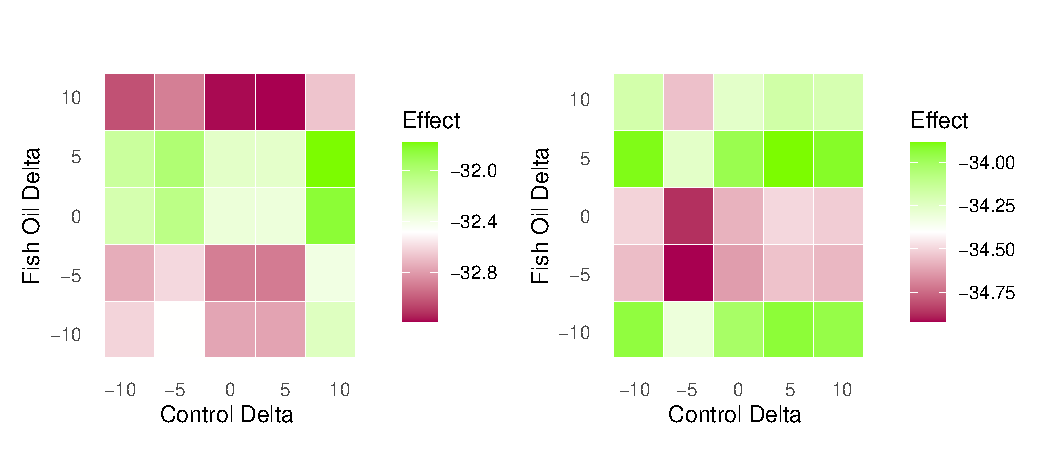
\includegraphics[keepaspectratio]{Final_Report_files/figure-latex/unnamed-chunk-36-1.pdf}}
\pandocbounded{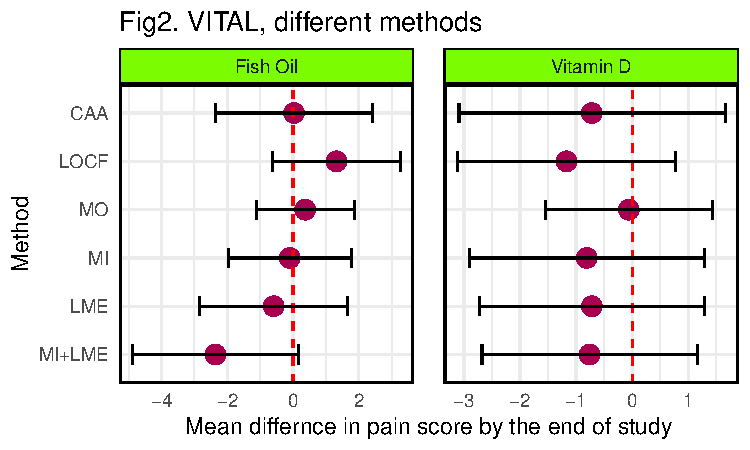
\includegraphics[keepaspectratio]{Final_Report_files/figure-latex/unnamed-chunk-36-2.pdf}}

Methods from top to bottom

\begin{itemize}
\item
  CAA: complete case analysis
\item
  LOCR: last observation carry forward
\item
  MO: mean observation
\item
  MI: multiple imputation and multiple linear regression
\item
  LME: linear mix model without imputations
\item
  MI+LME: multiple imputation and linear mix model
\end{itemize}

\subsection{Changing estimand}\label{changing-estimand}

In this section, we explore how changing the estimand (how time is
modeled) to see how that affects our conclusions.

\pandocbounded{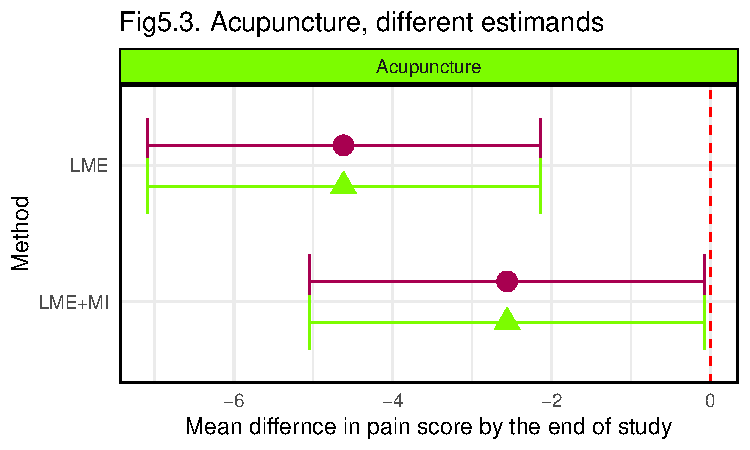
\includegraphics[keepaspectratio]{Final_Report_files/figure-latex/unnamed-chunk-37-1.pdf}}
\pandocbounded{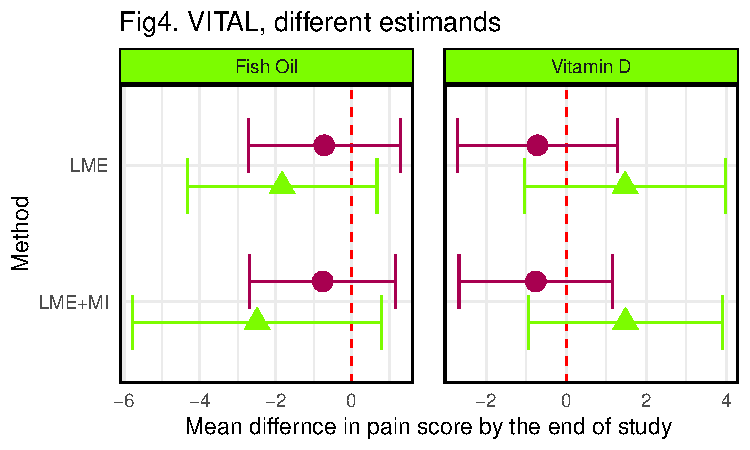
\includegraphics[keepaspectratio]{Final_Report_files/figure-latex/unnamed-chunk-37-2.pdf}}

Method on top: LME: linear mix model without imputations

Method on bottom: MI+LME: multiple imputation and linear miex model

Purple line (Reference) estimand: The mean difference of pain score at
the end of study, treating time as categorical variable

Green line (Changed) estimand: The mean difference of pain score at the
end of study, treating time as continuous variable

\subsection{Changing imputation methods and imputation
numbers}\label{changing-imputation-methods-and-imputation-numbers}

In this session. We keep our estimand treating time as a categorical
variable and using multiple linear regression as substantive model.

We first compared different imputation methods within the FCS framework,
using 5 imputations.

\pandocbounded{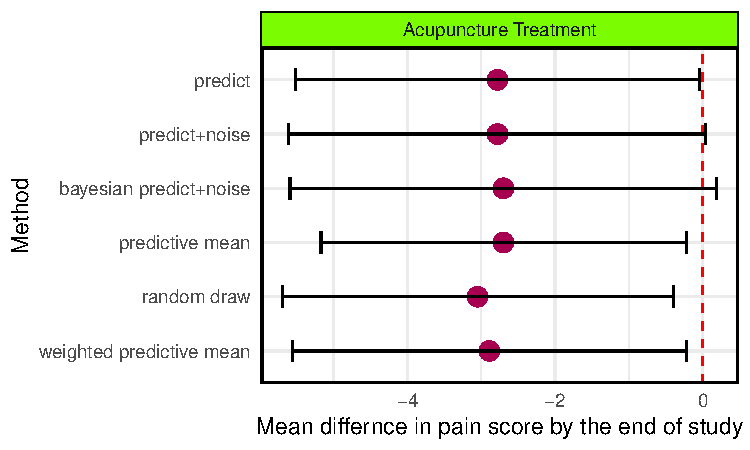
\includegraphics[keepaspectratio]{Final_Report_files/figure-latex/unnamed-chunk-38-1.pdf}}
\pandocbounded{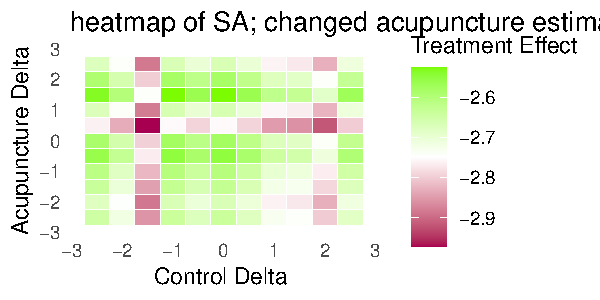
\includegraphics[keepaspectratio]{Final_Report_files/figure-latex/unnamed-chunk-38-2.pdf}}

Next, we assess the impact of changing the number of imputations, using
predictive mean method.

\pandocbounded{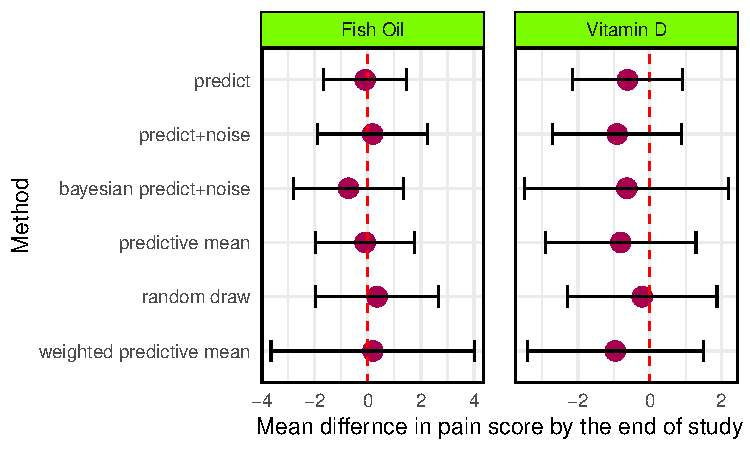
\includegraphics[keepaspectratio]{Final_Report_files/figure-latex/unnamed-chunk-39-1.pdf}}
\pandocbounded{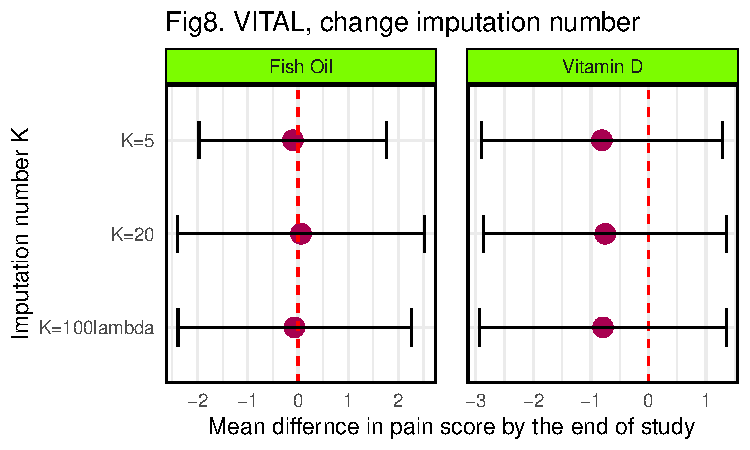
\includegraphics[keepaspectratio]{Final_Report_files/figure-latex/unnamed-chunk-39-2.pdf}}

\subsection{Sensitive analysis}\label{sensitive-analysis}

\pandocbounded{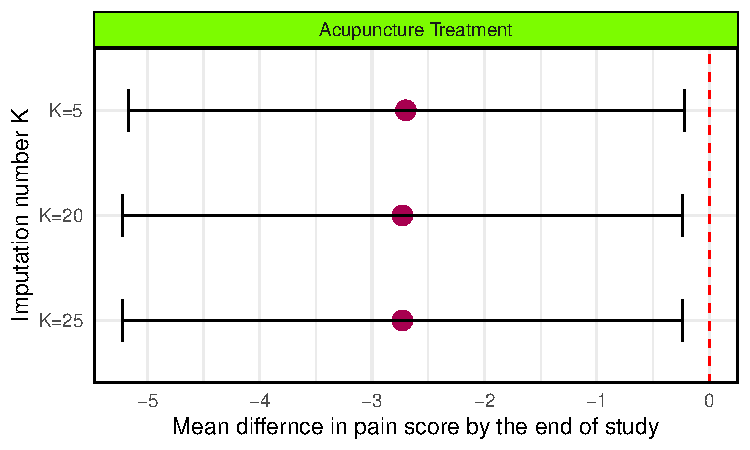
\includegraphics[keepaspectratio]{Final_Report_files/figure-latex/unnamed-chunk-40-1.pdf}}
\pandocbounded{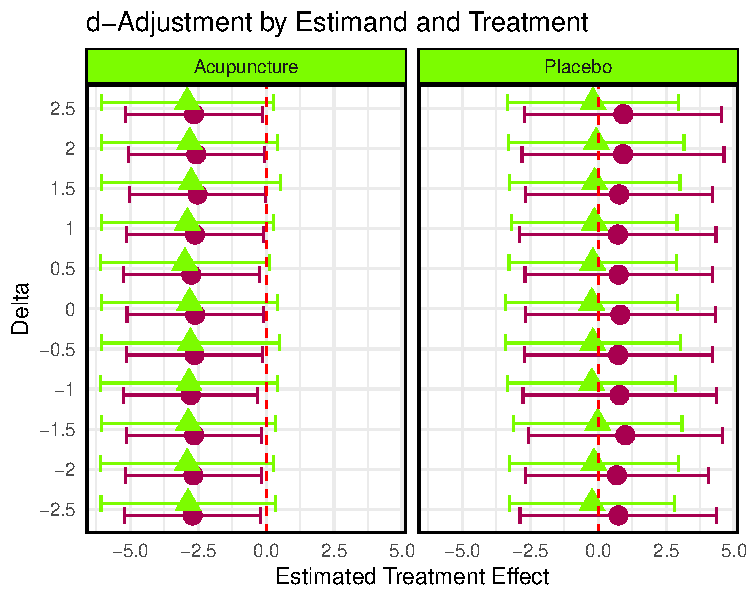
\includegraphics[keepaspectratio]{Final_Report_files/figure-latex/unnamed-chunk-40-2.pdf}}

This forest plot illustrates the robustness of the estimated treatment
effects under varying missing data assumptions using
\(\delta\)-adjustment. Each point represents the estimated treatment
effect at a given \(\delta\) value, where:

\begin{itemize}
\tightlist
\item
  Purple represent the reference estimand, in which time is treated as a
  categorical variable.
\item
  Green represent the changed estimand, in which time is modeled as a
  continuous variable.
\item
  Horizontal lines denote the 95\% confidence intervals.
\end{itemize}

The vertical red dashed line at 0 marks the threshold of no treatment
effect. The panels are stratified to compare the acupuncture group and
the control group in figure x. This goes for the VITAL plot in figure y
as well where we compare fish oil, vitamin D and control group. The
\(\delta\) parameter shifts the imputed values to simulate scenarios
where missing outcomes are systematically better or worse than observed
ones. Positive \(\delta\) values imply better unobserved outcomes;
negative \(\delta\) values imply worse. The consistency of effect
estimates across the \(\delta\) range suggests the treatment effect is
robust to departures from the MAR assumption.

\newpage

\pandocbounded{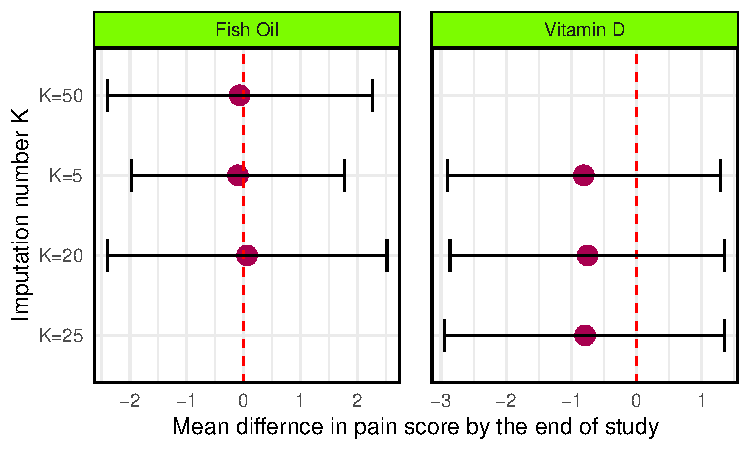
\includegraphics[keepaspectratio]{Final_Report_files/figure-latex/unnamed-chunk-41-1.pdf}}
\pandocbounded{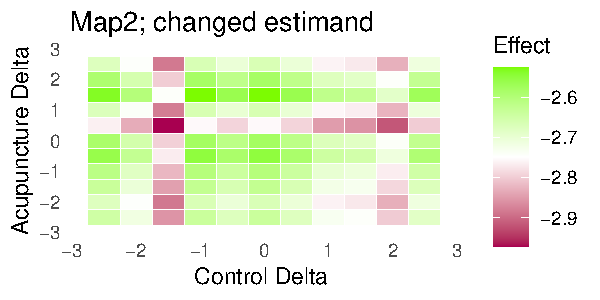
\includegraphics[keepaspectratio]{Final_Report_files/figure-latex/unnamed-chunk-41-2.pdf}}
\pandocbounded{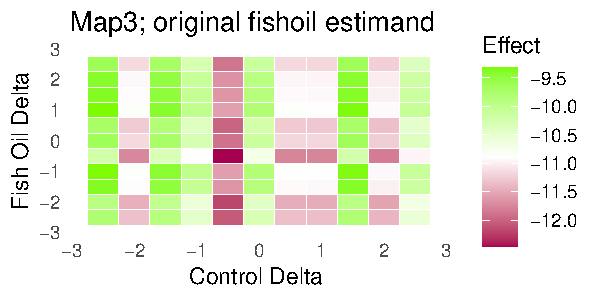
\includegraphics[keepaspectratio]{Final_Report_files/figure-latex/unnamed-chunk-41-3.pdf}}
\pandocbounded{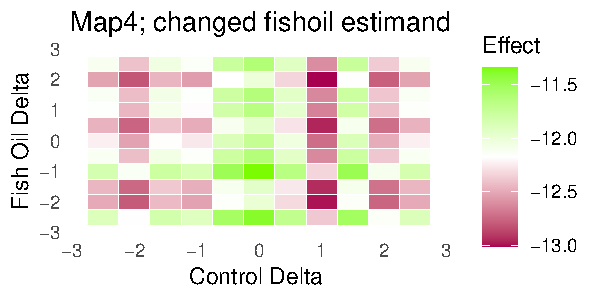
\includegraphics[keepaspectratio]{Final_Report_files/figure-latex/unnamed-chunk-41-4.pdf}}
\pandocbounded{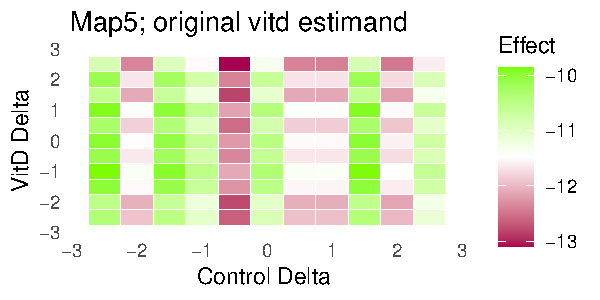
\includegraphics[keepaspectratio]{Final_Report_files/figure-latex/unnamed-chunk-41-5.pdf}}
\pandocbounded{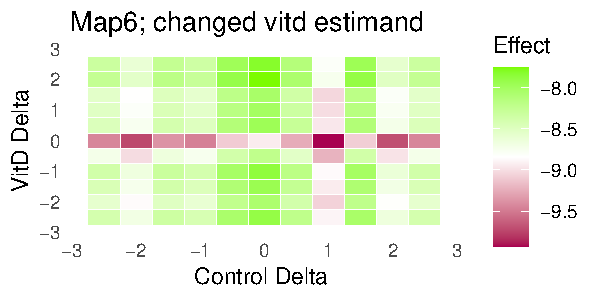
\includegraphics[keepaspectratio]{Final_Report_files/figure-latex/unnamed-chunk-41-6.pdf}}

We created heatmaps plotting the \(\delta\) values for both the control
group and treatment group to visualise the change in treatment effect
when varying the \(\delta\) adjustments under MNAR. The aim here is to
show the robustness of the initial estimated treatment effect when
assumed under a different mechanism. A similar range of colours would be
interpretable as a strong estimate as there was not much change in the
estimate after adding the \(\delta\) shifts.

\section{Discussion}\label{discussion}

Across all analyses, no meaningful difference was observed in the final
treatment effect estimates across the various methods and settings
explored.

However, several points are worth noting:

\begin{itemize}
\item
  In Figures 1 and 2, we observe that methods involving multiple
  imputation (MI) show more variation in the estimated treatment
  effects. This is expected, as MI leverages all available observed
  data, while the other four methods (CAA, LOCF, MO, and LME without
  imputation) use only a subset---typically including only group and
  baseline pain score.
\item
  When we changed the estimand to treat time as a continuous variable,
  the impact was minimal in the Acupuncture study, which is unsurprising
  given that it includes only two follow-up time points. In such cases,
  modeling time continuously offers limited additional information.
\end{itemize}

It is important to emphasize that the goal of this project is not to
revise prior conclusions from the original studies, but rather to gain
practical insights by applying and comparing different methods for
handling missing data.

The fact that our results are broadly consistent across methods should
not be taken to imply that simpler approaches like complete case
analysis (CAA) are equivalent to more principled methods. Even in a
similar future study, the same results may not hold, especially under
different missing data patterns or assumptions.

This project has highlighted that there are many valid approaches to
handling missing data, and that these can be combined in different ways
depending on the context. It is crucial to understand which methods are
most appropriate under which conditions.

For example:

\begin{itemize}
\item
  LME is a powerful tool for analyzing longitudinal data and can yield
  unbiased results even without imputation---if the assumptions are met.
  However, in the Acupuncture dataset, its utility is limited due to the
  small number of timepoints and its inability to incorporate auxiliary
  variables like pain frequency.
\item
  In the VITAL dataset, although there are more timepoints, baseline
  pain scores are sometimes missing. As a result, when fitting LME
  without imputation, those individuals are excluded. The exclusion
  number will be much higher when more covariates with missing data are
  added to the model, as any individuals with any baseline missing will
  be removed, potentially leading to substantial loss of information.
\end{itemize}

\subsection{Limitations of the
project}\label{limitations-of-the-project}

There are several limitations stemming from the inherent characteristics
of the datasets used in this project.These limitations are not a result
of analytic choices but rather reflect the practical boundaries of the
available data.

\begin{itemize}
\item
  \emph{Limited follow-up in Acupuncture dataset:} The Acupuncture study
  includes only two follow-up timepoints (3 and 12 months), which limits
  the ability to model time flexibly or detect subtle longitudinal
  trends. As a result, methods like linear mixed-effects models offer
  limited additional benefit in this context.
\item
  \emph{Weak treatment effect in VITAL:} The VITAL dataset shows
  relatively small therapeutic effects, making it difficult to detect
  meaningful differences between methods. This also reduces the
  practical impact of using more advanced imputation strategies.
\item
  \emph{No access to the full complete data:} Since we only work with
  partially observed datasets, we cannot assess the true accuracy of
  different imputation methods. Having access to fully observed data
  would allow direct comparison between imputed and actual values.
\end{itemize}

\subsection{Future work}\label{future-work}

In addition, there are methodological aspects that could be improved or
explored further in future work. These include choices related to model
specification, variable adjustment, and the diversity of imputation
techniques employed. Addressing these areas could enhance the robustness
and generalizability of findings, especially in more complex or
data-rich clinical contexts.

\begin{itemize}
\item
  \emph{Model specification:} Both linear regression and LME assume
  linearity and normally distributed residuals. These assumptions were
  not formally tested, and violations (e.g., non-linearity or skewness
  in outcome) could compromise model validity.
\item
  \emph{Single imputation method for main analysis:} While different
  imputation methods were explored, the main analyses relied on
  predictive mean matching. Other valid methods (e.g., Bayesian ridge
  regression, classification models for categorical variables) were not
  applied or compared in depth.
\item
  \emph{Limited covariate adjustment:} In all models, we only adjusted
  for treatment group and baseline pain score. While this was done for
  comparability across methods, it may limit model performance and bias
  control, particularly if other relevant covariates are predictive of
  missingness or outcomes.
\end{itemize}

\bibliographystyle{unsrt}
\bibliography{references.bib}


\end{document}
